%%%%%%%%%%%%%%%%%%%%%%%%%%%%%%%%%%%%%%%%%%%%%%%%%%%
\begin{frame}
  \begin{center}
    {\Large Recurrent Neural Network}
  \end{center}
\end{frame}

%%%%%%%%%%%%%%%%%%%%%%%%%%%%%%%%%%%%%%%%%%%%%%%%%%%
\begin{frame}[fragile] \frametitle{Toy Example: Scenario I: Cook: (Ref: Luis Serrano)}
An ideal roommate who cooks:
\begin{itemize}
\item Can cook 3 dishes: Apple Pie, Burger, Chicken
\item Dish depends on the outside weather (only Sunny or Rainy)
\begin{itemize}
\item Sunny: Apple Pie
\item Rainy: Burger
\end{itemize}
\end{itemize}
This can be easily modeled as Neural network with known inputs and outputs.
\end{frame}

%%%%%%%%%%%%%%%%%%%%%%%%%%%%%%%%%%%%%%%%%%%%%%%%%%%
\begin{frame}[fragile] \frametitle{Toy Example: Scenario I}
Lets model food and weather as one-hot encoding vectors
\begin{center}
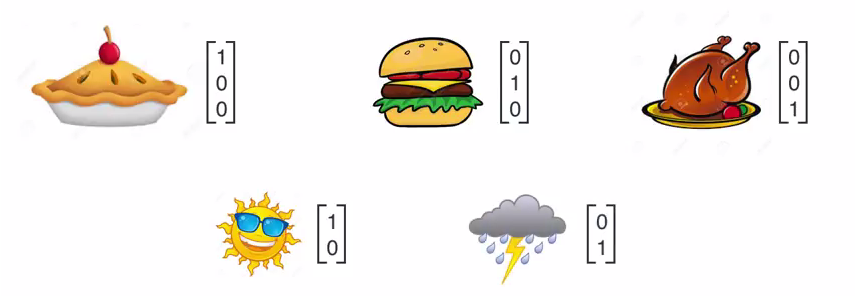
\includegraphics[width=\linewidth,keepaspectratio]{rnn6}
\end{center}
Network takes weather vector in and outputs food vector
\end{frame}

%%%%%%%%%%%%%%%%%%%%%%%%%%%%%%%%%%%%%%%%%%%%%%%%%%%
\begin{frame}[fragile] \frametitle{Toy Example: Scenario I}
\begin{itemize}
\item This Neural Network is represented by a matrix (3x2)g
\item Individual weather vector when post multiplies this matrix, resultant 3x1 vector represents food
\item For Sunny, you get Apple Pie
\item For Rainy, you get Burger.
\end{itemize}
\begin{center}
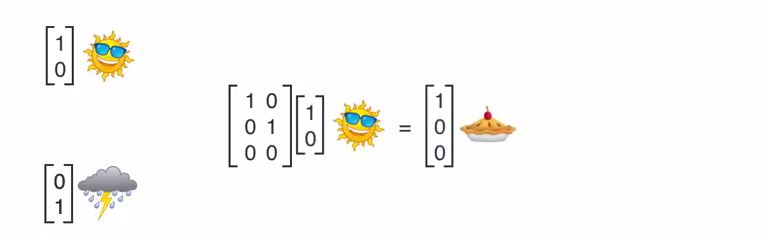
\includegraphics[width=\linewidth,keepaspectratio]{rnn7}
\end{center}
\end{frame}

%%%%%%%%%%%%%%%%%%%%%%%%%%%%%%%%%%%%%%%%%%%%%%%%%%%
\begin{frame}[fragile] \frametitle{Toy Example: Scenario I}
\begin{itemize}
\item Matrix can be seen as network as well.
\item First node emits 3 rays, each to each output node: 1, 0, 1. This is nothing but first column of the matrix
\item Second node emits 3 rays, each to each output node: 0, 1, 0. This is nothing but second column of the matrix
\item Input weather vector values are put into input nodes, multiplication happens and then output values are generated.
\end{itemize}
\begin{center}
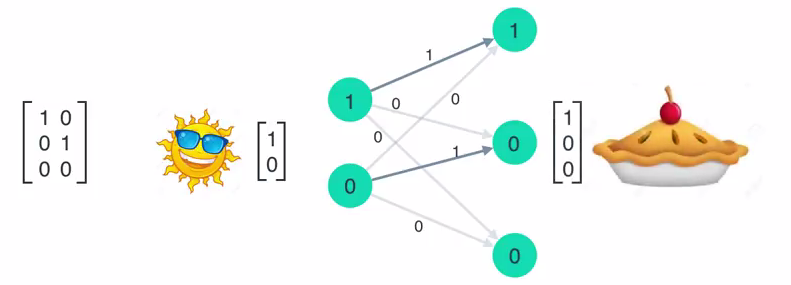
\includegraphics[width=0.8\linewidth,keepaspectratio]{rnn8}
\end{center}
\end{frame}

%%%%%%%%%%%%%%%%%%%%%%%%%%%%%%%%%%%%%%%%%%%%%%%%%%%
\begin{frame}[fragile] \frametitle{Toy Example: Scenario II}

\begin{itemize}
\item Same roommate, but instead of weather he decides the dish based on previous day.
\item One day Apple Pie, next Burger, next Chicken.
\end{itemize}
\begin{center}
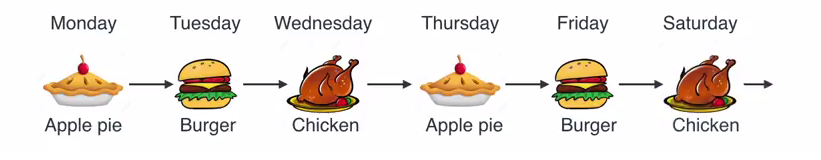
\includegraphics[width=\linewidth,keepaspectratio]{rnn9}
\end{center}
\end{frame}

%%%%%%%%%%%%%%%%%%%%%%%%%%%%%%%%%%%%%%%%%%%%%%%%%%%
\begin{frame}[fragile] \frametitle{Toy Example: Scenario II}

\begin{itemize}
\item This is not normal Neural network, its called Recurrent Neural Network (RNN)
\item There is no Weather input, but previous day's output is its input. Shown as loop.
\end{itemize}
\begin{center}
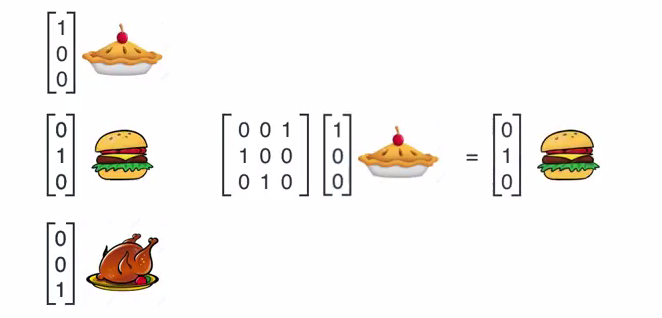
\includegraphics[width=0.8\linewidth,keepaspectratio]{rnn10}
\end{center}
\end{frame}


%%%%%%%%%%%%%%%%%%%%%%%%%%%%%%%%%%%%%%%%%%%%%%%%%%%
\begin{frame}[fragile] \frametitle{Toy Example: Scenario II}
As a network:
\begin{itemize}
\item 3 inputs, 3 outputs
\item Both representing food
\item Its basically looping back. So, its Recurrent.
\end{itemize}
\begin{center}
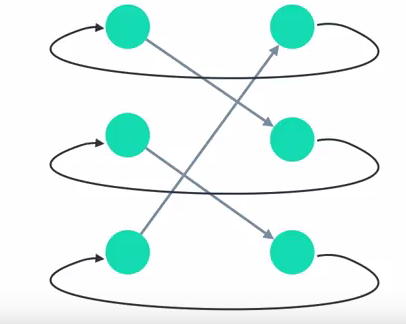
\includegraphics[width=0.5\linewidth,keepaspectratio]{rnn11}
\end{center}
\end{frame}

%%%%%%%%%%%%%%%%%%%%%%%%%%%%%%%%%%%%%%%%%%%%%%%%%%%
\begin{frame}[fragile] \frametitle{Toy Example: Scenario III}
\begin{itemize}
\item Same roommate, but now the rules of cooking are dependent on both, weather as well as previous day dish
\item If Sunny, he goes out, has fun, no cooking, so dish is leftover, same as yesterday
\item If Rainy, he is at home, next dish on the sequence.
\item Below, for Tuesday, it's Sunny weather is shown under Monday (just for illustration) as input
\end{itemize}
\begin{center}
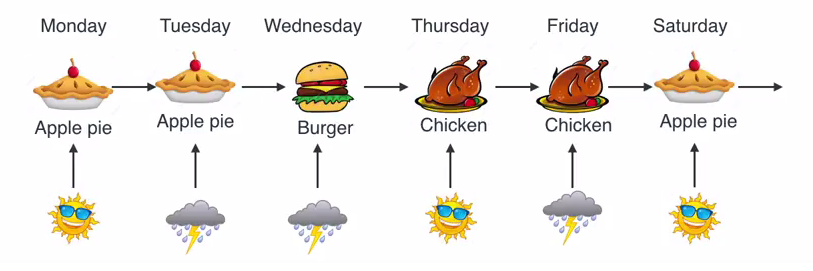
\includegraphics[width=0.8\linewidth,keepaspectratio]{rnn12}
\end{center}
\end{frame}


%%%%%%%%%%%%%%%%%%%%%%%%%%%%%%%%%%%%%%%%%%%%%%%%%%%
\begin{frame}[fragile] \frametitle{Toy Example: Scenario III}
Food Matrix
\begin{itemize}
\item Food matrix artificially cut into two
\item Top represents Sunny, bottom as Rainy
\item Apple Pie comes in, top results in Apple Pie as TODAY's food (same), bottom results in next dish, ToMORROW's food.
\item Nothing about Weather as of now.
\end{itemize}
\begin{center}
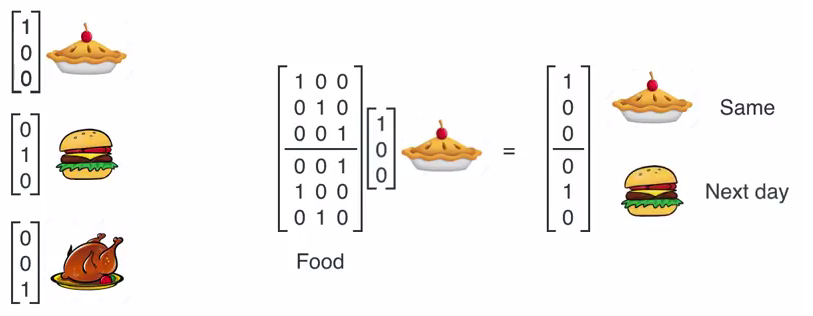
\includegraphics[width=0.8\linewidth,keepaspectratio]{rnn13}
\end{center}
\end{frame}

%%%%%%%%%%%%%%%%%%%%%%%%%%%%%%%%%%%%%%%%%%%%%%%%%%%
\begin{frame}[fragile] \frametitle{Toy Example: Scenario III}
Weather Matrix
\begin{itemize}
\item Top results are all 1's. Same as Today, Sunny as 1 represents Sunny, 0 Rainy.
\item Bottom result are all 0's. For Next day.
\item Weather matrix tells, if he as to cook TODAY's food or TOMORROW's food. As the bottom results are all 1's, or YES's.
\end{itemize}
\begin{center}
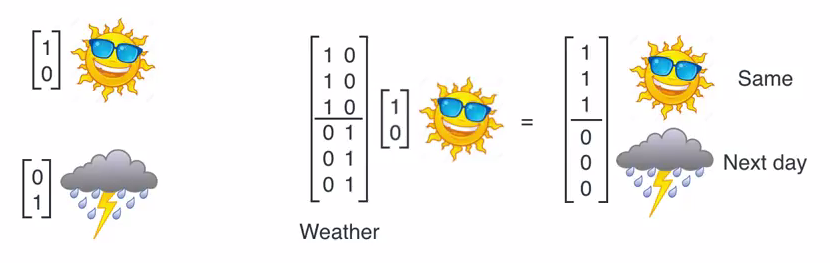
\includegraphics[width=0.8\linewidth,keepaspectratio]{rnn14}
\end{center}
\end{frame}

%%%%%%%%%%%%%%%%%%%%%%%%%%%%%%%%%%%%%%%%%%%%%%%%%%%
\begin{frame}[fragile] \frametitle{Toy Example: Scenario III}
\begin{itemize}
\item Combining two matrices should give clear signal on what to cook.
\item Food Matrix: Whats the food for today? Whats for tomorrow?
\item Weather Matrix: Should I cook today? or tomorrow?
\end{itemize}
\begin{center}
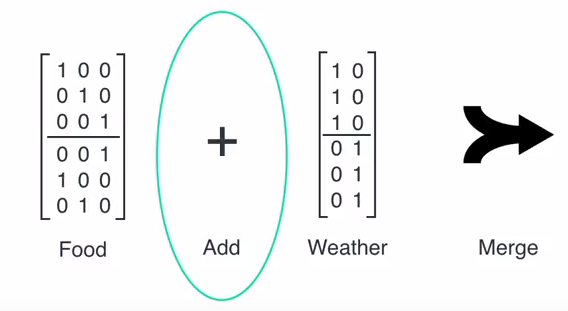
\includegraphics[width=0.8\linewidth,keepaspectratio]{rnn15}
\end{center}
\end{frame}


%%%%%%%%%%%%%%%%%%%%%%%%%%%%%%%%%%%%%%%%%%%%%%%%%%%
\begin{frame}[fragile] \frametitle{Toy Example: Scenario III}
Testing
\begin{itemize}
\item Say, we had Apple Pie yesterday and its rainy today
\item Food Matrix is computed and added to Weather Matrix
\end{itemize}
\begin{center}
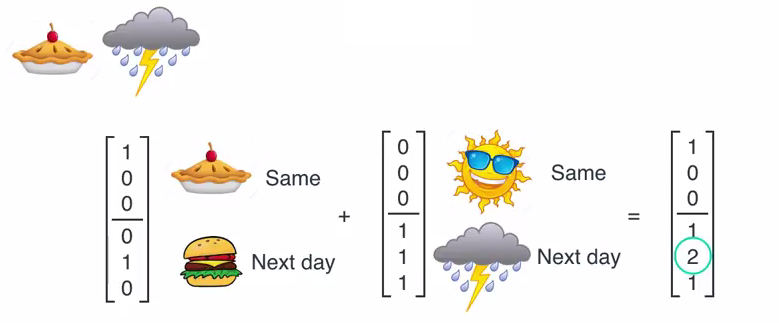
\includegraphics[width=0.8\linewidth,keepaspectratio]{rnn16}
\end{center}
\end{frame}

%%%%%%%%%%%%%%%%%%%%%%%%%%%%%%%%%%%%%%%%%%%%%%%%%%%
\begin{frame}[fragile] \frametitle{Toy Example: Scenario III}
Merge
\begin{itemize}
\item We apply non linear function that takes input of the combined results
\item Maps it to uniform one-hot like result.
\item It make the LARGEST as 1, else all to 0
\item Add sub-components  and produces the result
\end{itemize}
\begin{center}
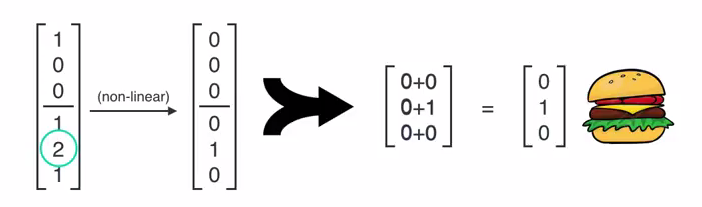
\includegraphics[width=0.8\linewidth,keepaspectratio]{rnn17}
\end{center}
\end{frame}

%%%%%%%%%%%%%%%%%%%%%%%%%%%%%%%%%%%%%%%%%%%%%%%%%%%
\begin{frame}[fragile] \frametitle{Toy Example: Scenario III}
Summary (shown arrows are 1)
\begin{center}
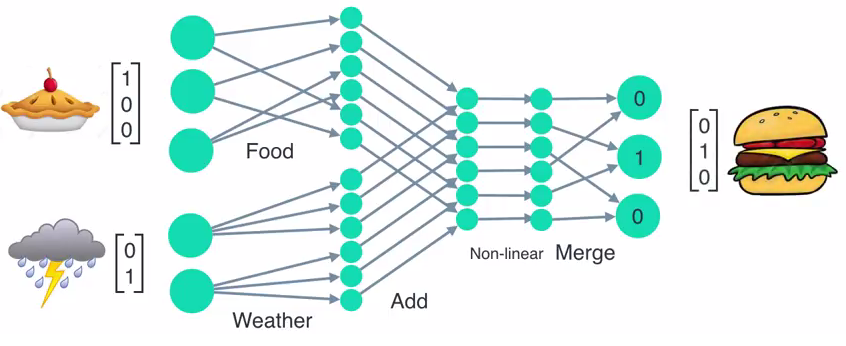
\includegraphics[width=\linewidth,keepaspectratio]{rnn18}
\end{center}
\end{frame}

%%%%%%%%%%%%%%%%%%%%%%%%%%%%%%%%%%%%%%%%%%%%%%%%%%%
\begin{frame}[fragile] \frametitle{Toy Example: Scenario III}
Recurrent
\begin{center}
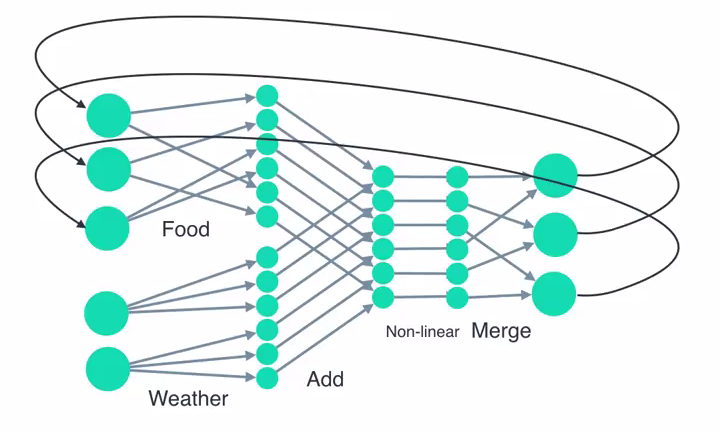
\includegraphics[width=\linewidth,keepaspectratio]{rnn19}
\end{center}
\end{frame}

%%%%%%%%%%%%%%%%%%%%%%%%%%%%%%%%%%%%%%%%%%%%%%%%%%%
\begin{frame}[fragile] \frametitle{Toy Example: Scenario IV: Summary}
\begin{itemize}
\item We can group together inputs and outputs.
\item Two inputs: yesterday's predictions and yesterday's dish
\item One output: today's prediction
\end{itemize}
\begin{center}
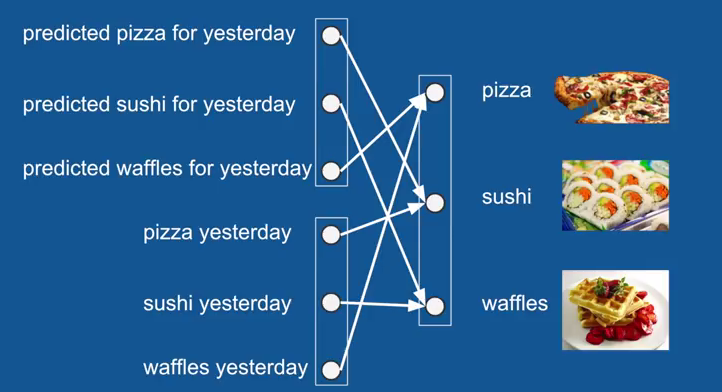
\includegraphics[width=0.8\linewidth,keepaspectratio]{rnn20}
\end{center}
\end{frame}

%%%%%%%%%%%%%%%%%%%%%%%%%%%%%%%%%%%%%%%%%%%%%%%%%%%
\begin{frame}[fragile] \frametitle{Toy Example: Scenario IV: Summary}
\begin{itemize}
\item Prediction is recycled as input
\item The dotted line, holds it to be used today
\end{itemize}
\begin{center}
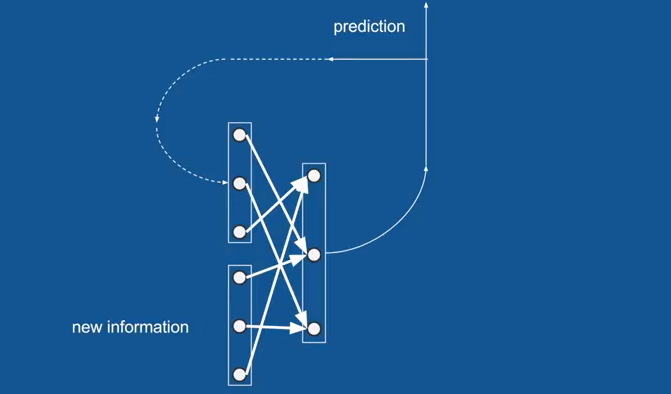
\includegraphics[width=0.8\linewidth,keepaspectratio]{rnn21}
\end{center}
\end{frame}

%%%%%%%%%%%%%%%%%%%%%%%%%%%%%%%%%%%%%%%%%%%%%%%%%%%
\begin{frame}[fragile] \frametitle{Toy Example: Scenario IV: Summary}
\begin{itemize}
\item So, even if we missed few time steps in between, 
\item We can play the actions forward from the known past time
\end{itemize}
\begin{center}
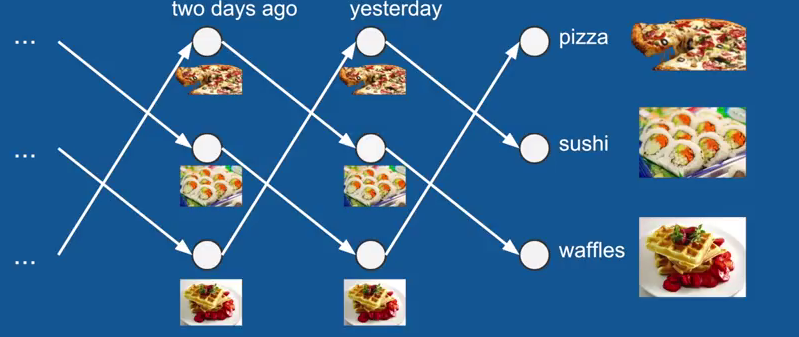
\includegraphics[width=0.8\linewidth,keepaspectratio]{rnn22}
\end{center}
\end{frame}

%%%%%%%%%%%%%%%%%%%%%%%%%%%%%%%%%%%%%%%%%%%%%%%%%%%
\begin{frame}[fragile] \frametitle{RNN}
\begin{itemize}
\item When data is sequential
\item Next depends on previous + extra input
\item Example: Stock Predictions, Language Model (next word prediction), etc.
\end{itemize}
\end{frame}





%%%%%%%%%%%%%%%%%%%%%%%%%%%%%%%%%%%%%%%%%%%%%%%%%%%
\begin{frame}[fragile] \frametitle{Recurrent neural networks}

A recurrent neural network can be thought of as multiple copies of the same network, each passing a message to a successor. 
The diagram above shows what happens if we unroll the loop. 

\begin{center}
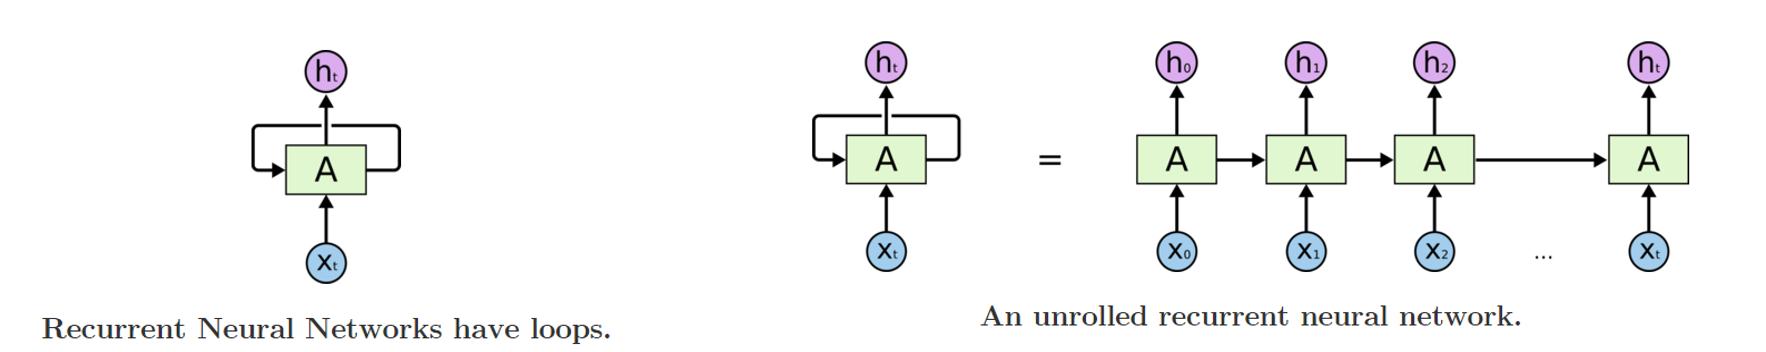
\includegraphics[width=0.8\linewidth,keepaspectratio]{rnn}
\end{center}
\end{frame}


%%%%%%%%%%%%%%%%%%%%%%%%%%%%%%%%%%%%%%%%%%%%%%%%%%%
\begin{frame}[fragile] \frametitle{Recurrent neural networks}
RNN allow us to operate over sequences of vectors. Many types
\begin{center}
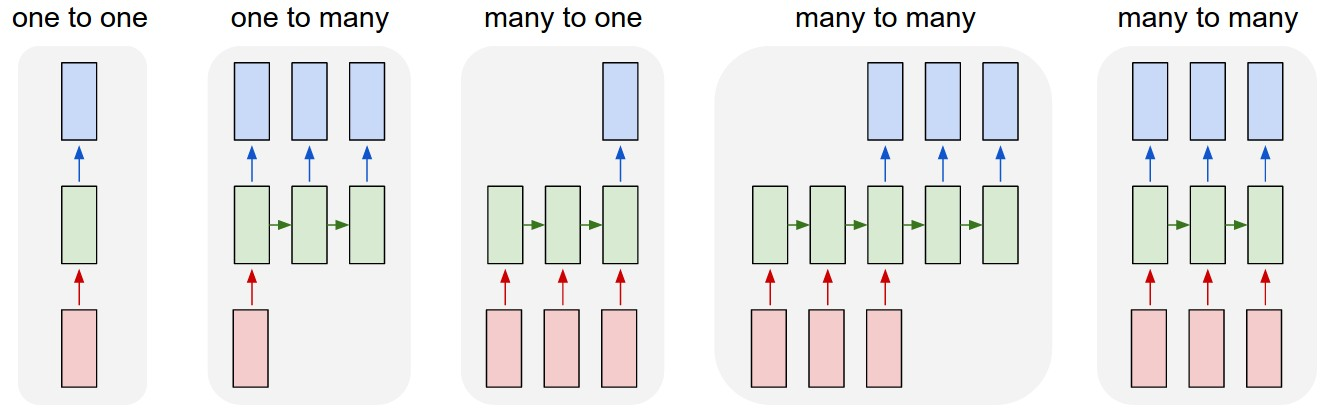
\includegraphics[width=0.8\linewidth,keepaspectratio]{rnn23}
\end{center}
Each rectangle is a vector and arrows represent functions (e.g. matrix multiply). Input vectors are in red, output vectors are in blue and green vectors hold the RNN's state
\end{frame}



%%%%%%%%%%%%%%%%%%%%%%%%%%%%%%%%%%%%%%%%%%%%%%%%%%%
\begin{frame}[fragile] \frametitle{Recurrent neural networks}
\begin{center}
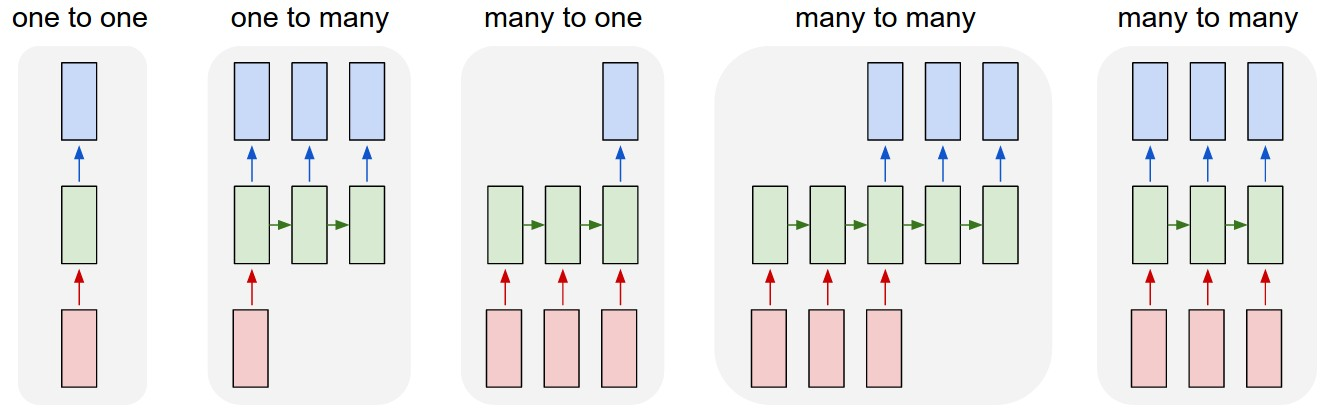
\includegraphics[width=0.8\linewidth,keepaspectratio]{rnn23}
\end{center}
One-to-One: Vanilla mode of processing without RNN, from fixed-sized input to fixed-sized output (e.g. image classification).
\end{frame}

%%%%%%%%%%%%%%%%%%%%%%%%%%%%%%%%%%%%%%%%%%%%%%%%%%%
\begin{frame}[fragile] \frametitle{Recurrent neural networks}
\begin{center}
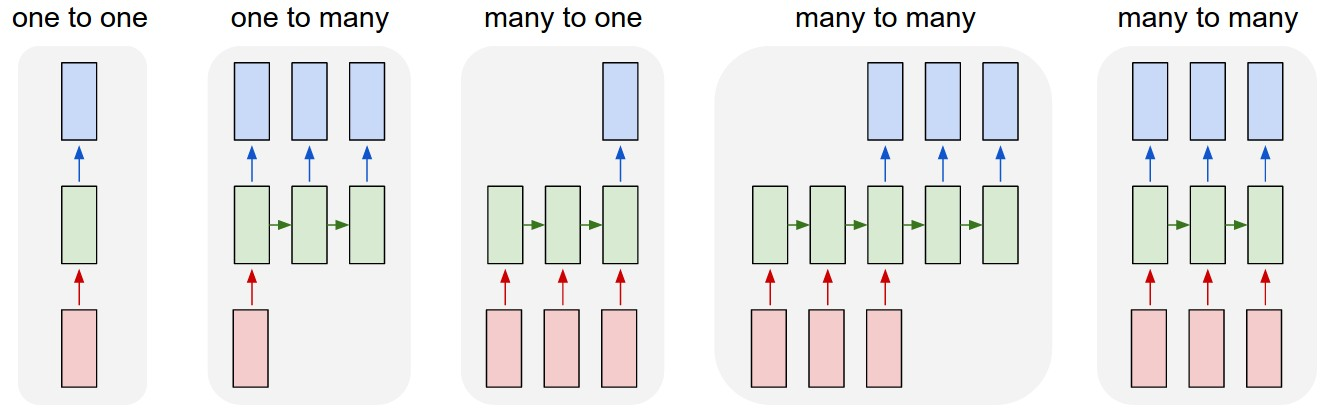
\includegraphics[width=0.8\linewidth,keepaspectratio]{rnn23}
\end{center}
One-to-Many: Sequence output (e.g. image captioning takes an image (fixed size) and outputs a sentence of words).
\end{frame}

%%%%%%%%%%%%%%%%%%%%%%%%%%%%%%%%%%%%%%%%%%%%%%%%%%%
\begin{frame}[fragile] \frametitle{Recurrent neural networks}
\begin{center}
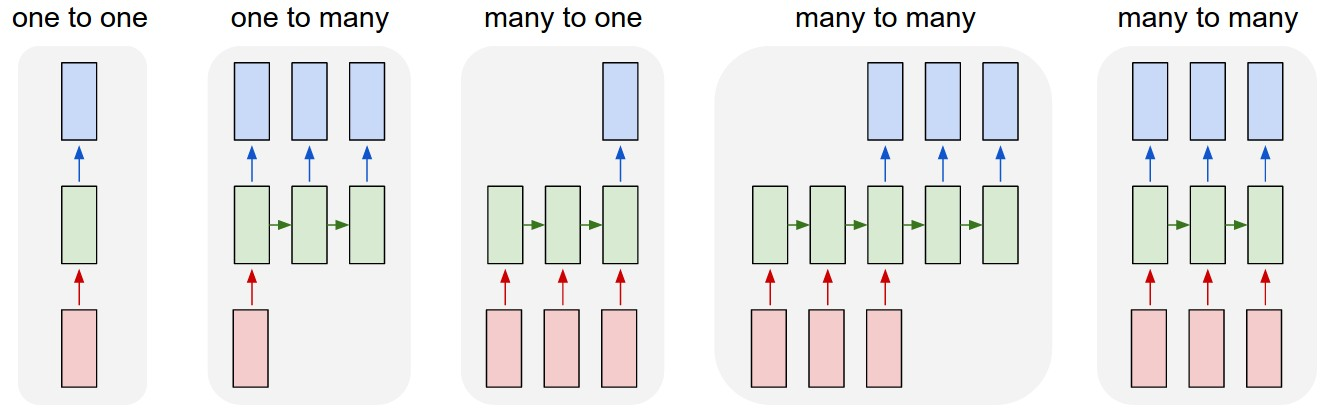
\includegraphics[width=0.8\linewidth,keepaspectratio]{rnn23}
\end{center}
One-to-Many: Sequence output (e.g. image captioning takes an image (fixed size) and outputs a sentence of words).
\end{frame}

%%%%%%%%%%%%%%%%%%%%%%%%%%%%%%%%%%%%%%%%%%%%%%%%%%%
\begin{frame}[fragile] \frametitle{Recurrent neural networks}
\begin{center}
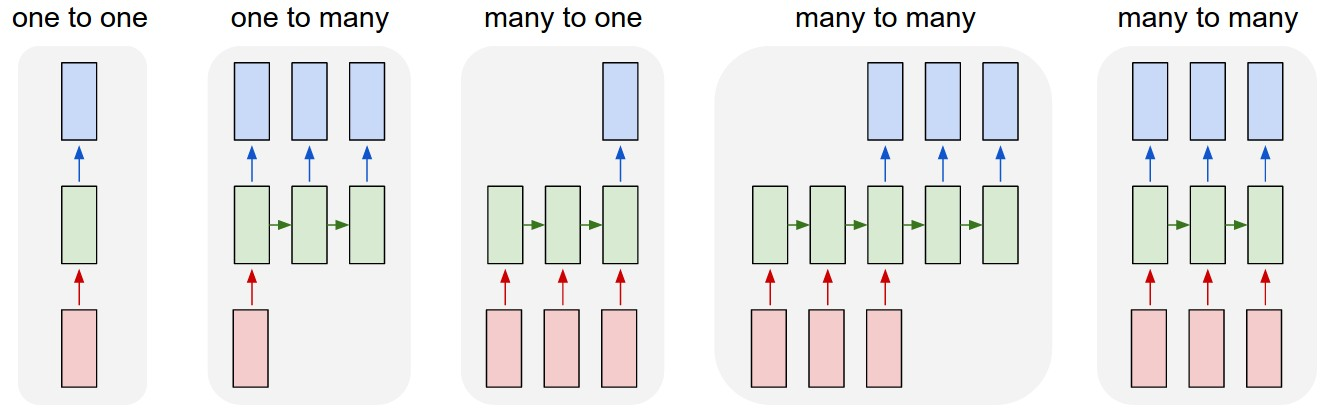
\includegraphics[width=0.8\linewidth,keepaspectratio]{rnn23}
\end{center}
Many-to-One: Sequence input (e.g. sentiment analysis where a given sentence is classified as expressing positive or negative sentiment).
\end{frame}

%%%%%%%%%%%%%%%%%%%%%%%%%%%%%%%%%%%%%%%%%%%%%%%%%%%
\begin{frame}[fragile] \frametitle{Recurrent neural networks}
\begin{center}
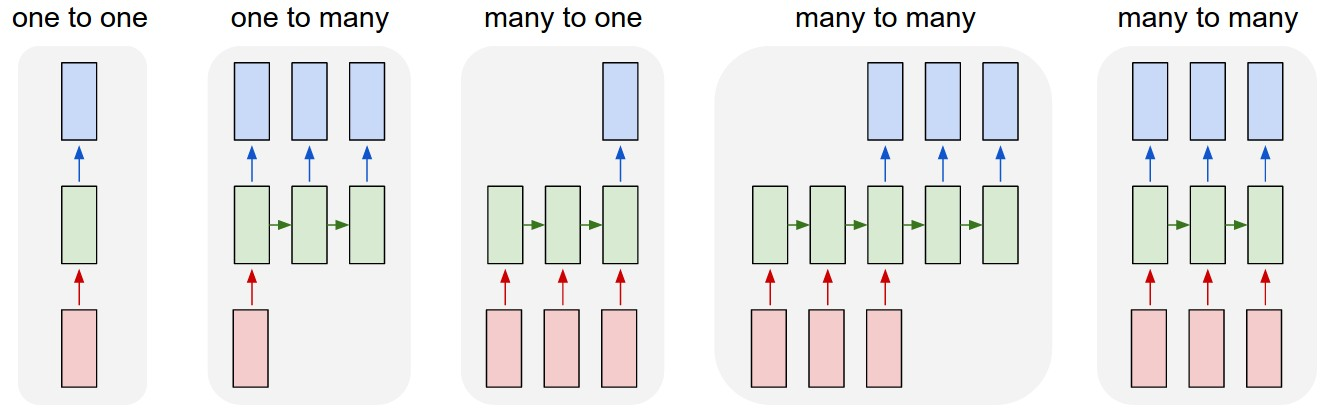
\includegraphics[width=0.8\linewidth,keepaspectratio]{rnn23}
\end{center}
Many-to-Many: Sequence input and sequence output (e.g. Machine Translation: an RNN reads a sentence in English and then outputs a sentence in French).
\end{frame}

%%%%%%%%%%%%%%%%%%%%%%%%%%%%%%%%%%%%%%%%%%%%%%%%%%%
\begin{frame}[fragile] \frametitle{Recurrent neural networks}
\begin{center}
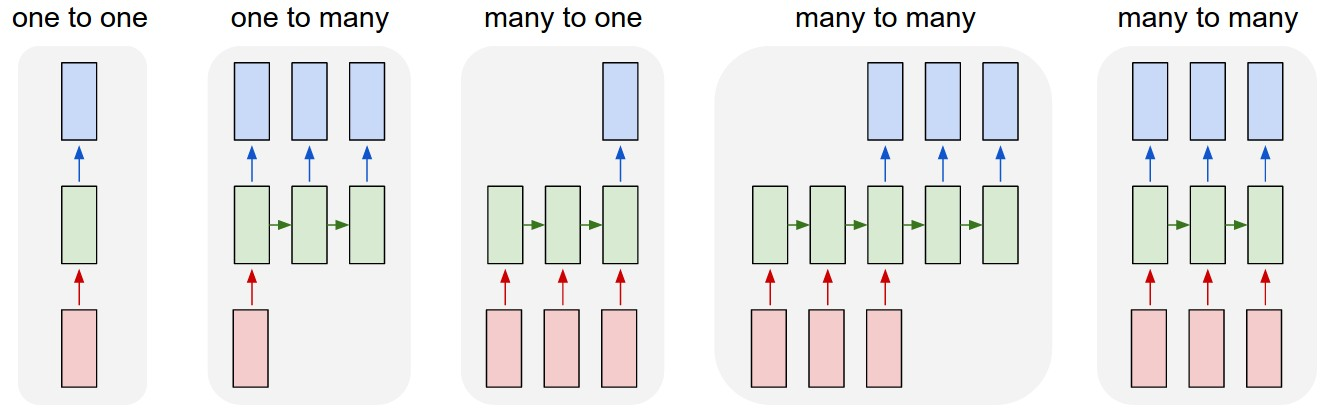
\includegraphics[width=0.8\linewidth,keepaspectratio]{rnn23}
\end{center}
Many-to-Many: Synced sequence input and output (e.g. video classification where we wish to label each frame of the video).
\end{frame}

%%%%%%%%%%%%%%%%%%%%%%%%%%%%%%%%%%%%%%%%%%%%%%%%%%%
\begin{frame}[fragile] \frametitle{Recurrent neural networks}
\begin{center}
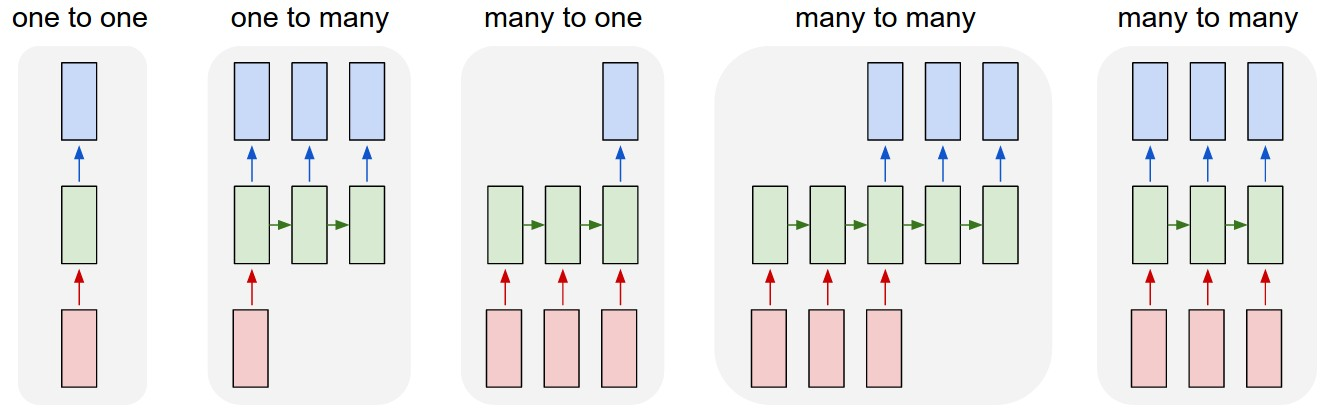
\includegraphics[width=0.8\linewidth,keepaspectratio]{rnn23}
\end{center}
Notice that in every case are no pre-specified constraints on the lengths sequences because the recurrent transformation (green) is fixed and can be applied as many times as we like.
\end{frame}



%%%%%%%%%%%%%%%%%%%%%%%%%%%%%%%%%%%%%%%%%%%%%%%%%%%
\begin{frame}[fragile] \frametitle{RNN: Sequential processing in absence of sequences.}
\begin{center}
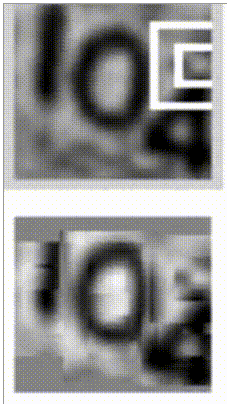
\includegraphics[width=0.3\linewidth,keepaspectratio]{rnn24}
\end{center}
Images are fixed size. But for sequential numbers in it, RNN learns to read out house numbers from left to right.
\end{frame}


%% http://karpathy.github.io/2015/05/21/rnn-effectiveness/
%% https://www.youtube.com/watch?v=iX5V1WpxxkY&index=10&list=LLsBKTrp45lTfHa_p49I2AEQ








%%%%%%%%%%%%%%%%%%%%%%%%%%%%%%%%%%%%%%%%%%%%%%%%%%%
\begin{frame}[fragile] \frametitle{RNNs Intuition}

\begin{itemize}
\item Human thoughts have persistence; humans don't start their thinking from scratch every second. 
\item As you read this sentence, you understand each word based on your understanding of previous words.  
\end{itemize}
\end{frame}

%%%%%%%%%%%%%%%%%%%%%%%%%%%%%%%%%%%%%%%%%%%%%%%%%%%
\begin{frame}[fragile] \frametitle{RNNs Intuition}

\begin{itemize}
\item One of the appeals of RNNs is the idea that they are able to connect previous information to the present task
\item E.g., using previous video frames to inform the understanding of the present frame.
\item E.g., a language model tries to predict the next word based on the previous ones.
\end{itemize}
\end{frame}

%%%%%%%%%%%%%%%%%%%%%%%%%%%%%%%%%%%%%%%%%%%%%%%%%%%
\begin{frame}[fragile] \frametitle{What is Neural Memory?}

\begin{itemize}
\item List the alphabet forward\ldots. you can do it, yes?
\item List the alphabet backward\ldots. hmmm\ldots perhaps a bit tougher.
\item Try with the lyrics of a song you know?
\item Why is it easier to recall forward than it is to recall backward? Can you jump into the middle of the second verse?\ldots hmm\ldots also difficult. Why?
\end{itemize}
\end{frame}

%%%%%%%%%%%%%%%%%%%%%%%%%%%%%%%%%%%%%%%%%%%%%%%%%%%
\begin{frame}[fragile] \frametitle{What is Neural Memory?}

\begin{itemize}
\item There's a very logical reason for this
\item You learned them as a sequence. 
\item You are really good at indexing from one letter to the next.
\item It's a kind of conditional memory. (Once you given a start of poem, you can recite it further)
\item All these  tasks are easier when you know what happened earlier in the sequence
\end{itemize}
\end{frame}

%%%%%%%%%%%%%%%%%%%%%%%%%%%%%%%%%%%%%%%%%%%%%%%%%%%
\begin{frame}[fragile] \frametitle{What is Neural Memory?}

\begin{itemize}
\item However, it's not that you don't have the song in your memory except when you're singing it. 
\item Instead, when you try to jump straight to the middle of the song, you simply have a hard time finding that representation in your brain (perhaps that set of neurons).
\item It starts searching all over looking for the middle of the song, but it hasn't tried to look for it this way before, so it doesn't have a map to the location of the middle of the second verse.
\end{itemize}
\end{frame}

%%%%%%%%%%%%%%%%%%%%%%%%%%%%%%%%%%%%%%%%%%%%%%%%%%%
\begin{frame}[fragile] \frametitle{What is Neural Memory?}

\begin{itemize}
\item If you wanted to train a neural network to predict whats the next scene would be in the next frame, it would be really helpful to know where the scene was in the last frame! 
\item Sequential data like this is why we build recurrent neural networks.
\end{itemize}
\end{frame}

%%%%%%%%%%%%%%%%%%%%%%%%%%%%%%%%%%%%%%%%%%%%%%%%%%%
\begin{frame}[fragile] \frametitle{What is Neural Memory?}

\begin{itemize}
\item Neural networks have hidden layers. Normally, the state of your hidden layer is based ONLY on your input data. 
\item So, normally a neural network's information flow would look like this:
$input \rightarrow hidden  \rightarrow  output$
\end{itemize}
\end{frame}


%%%%%%%%%%%%%%%%%%%%%%%%%%%%%%%%%%%%%%%%%%%%%%%%%%%
\begin{frame}[fragile] \frametitle{What is Neural Memory?}

\begin{itemize}
\item This is straightforward. Certain types of input create certain types of hidden layers. 
\item Certain types of hidden layers create certain types of output layers. 
\item It's kind-of a closed system. Memory changes this. 
\end{itemize}
\end{frame}


%%%%%%%%%%%%%%%%%%%%%%%%%%%%%%%%%%%%%%%%%%%%%%%%%%%
\begin{frame}[fragile] \frametitle{What is Neural Memory?}
\begin{itemize}
\item Memory means that the hidden layer is a combination of your input data at the current time-step and the hidden layer of the previous timestep.
$ (input + prev\_hidden) \rightarrow hidden \rightarrow output$
\item Why the hidden layer? Well, we could technically do this. 
$(input + prev\_input) \rightarrow hidden \rightarrow output$
\end{itemize}
\end{frame}

%%%%%%%%%%%%%%%%%%%%%%%%%%%%%%%%%%%%%%%%%%%%%%%%%%%
\begin{frame}[fragile] \frametitle{What is Neural Memory?}
Here, we have 4 timesteps of a recurrent neural network pulling information from the previous hidden layer.
\begin{itemize}
\item $(input + empty\_hidden) \rightarrow hidden \rightarrow output$
\item $(input + prev\_hidden) \rightarrow hidden \rightarrow output$
\item $(input + prev\_hidden) \rightarrow hidden \rightarrow output$
\item $(input + prev\_hidden) \rightarrow hidden \rightarrow output$
\end{itemize}
\end{frame}

%%%%%%%%%%%%%%%%%%%%%%%%%%%%%%%%%%%%%%%%%%%%%%%%%%%
\begin{frame}[fragile] \frametitle{What is Neural Memory?}
Colored show how hidden layer gets updated. 
4 timesteps with hidden layer recurrence:
\begin{center}
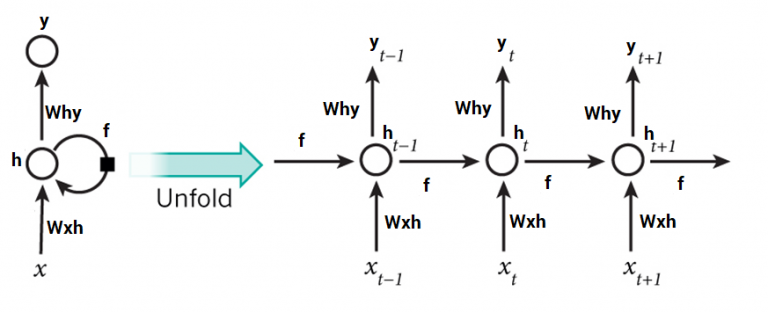
\includegraphics[width=0.6\linewidth,keepaspectratio]{rnn1}
\end{center}
4 timesteps with input  layer recurrence:
\begin{center}
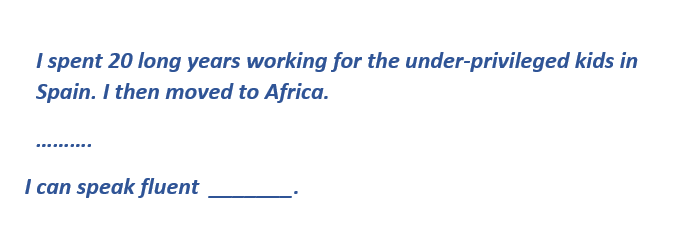
\includegraphics[width=0.6\linewidth,keepaspectratio]{rnn2}
\end{center}
Focus on the last hidden layer (4th line).
\end{frame}

%%%%%%%%%%%%%%%%%%%%%%%%%%%%%%%%%%%%%%%%%%%%%%%%%%%
\begin{frame}[fragile] \frametitle{What is Neural Memory?}
\begin{itemize}
\item  In the hidden layer recurrence, we see a presence of every input seen so far. In the input layer recurrence, it's exclusively defined by the current and previous inputs. 
\item This is why we model hidden recurrence.
\item Hidden recurrence learns what to remember whereas input recurrence is hard wired to just remember the immediately previous datapoint. 
\end{itemize}
\end{frame}

%%%%%%%%%%%%%%%%%%%%%%%%%%%%%%%%%%%%%%%%%%%%%%%%%%%
\begin{frame}[fragile] \frametitle{What is Neural Memory?}
\begin{itemize}
\item  Now compare and contrast these two approaches with the backwards alphabet and middle-of-song exercises. 
\item The hidden layer is constantly changing as it gets more inputs. 
\item Furthermore, the only way that we could reach these hidden states is with the correct sequence of inputs.
\end{itemize}
\end{frame}



%%%%%%%%%%%%%%%%%%%%%%%%%%%%%%%%%%%%%%%%%%%%%%%%%%%
\begin{frame}[fragile] \frametitle{What is Neural Memory?}
\begin{itemize}
\item  What's the practical difference? Let's say we were trying to predict the next word in a song given the previous. 
\item The ``input layer recurrence'' would break down if the song accidentally had the same sequence of two words in multiple places. 
\item Think about it, if the song had the statements ''I love you'', and ''I love carrots'', and the network was trying to predict the next word, how would it know what follows ''I love''? 
It could be carrots. It could be you. The network REALLY needs to know more about what part of the song its in.
\end{itemize}
\end{frame}


%%%%%%%%%%%%%%%%%%%%%%%%%%%%%%%%%%%%%%%%%%%%%%%%%%%
\begin{frame}[fragile] \frametitle{What is Neural Memory?}
\begin{itemize}
\item  It could be carrots. 
\item It could be you. 
\item The network REALLY needs to know more about what part of the song its in.
\item However, the ''hidden layer recurrence'' doesn't break down in this way. 
\item It subtely remembers everything it saw (with memories becoming more subtle as it they fade into the past).
\end{itemize}
\end{frame}


%%%%%%%%%%%%%%%%%%%%%%%%%%%%%%%%%%%%%%%%%%%%%%%%%%%
\begin{frame}[fragile] \frametitle{RNN - Neural Network Memory}
Normal NN process:
\begin{itemize}
\item Our input layer to the neural network is determined by our input dataset. 
\item Each row of input data is used to generate the hidden layer (via forward propagation). 
\item Each hidden layer is then used to populate the output layer (assuming only 1 hidden layer)
\end{itemize}
\end{frame}


%%%%%%%%%%%%%%%%%%%%%%%%%%%%%%%%%%%%%%%%%%%%%%%%%%%
\begin{frame}[fragile] \frametitle{RNN - Neural Network Memory}
\begin{itemize}
\item Just saw, memory means that the hidden layer is a combination of the input data and the previous hidden layer. 
\item How is this done?
\item Much like every other propagation in neural networks, it's done with a matrix. 
\item This matrix defines the relationship between the previous hidden layer and the current one.
\end{itemize}
\end{frame}

%%%
%%%%%%%%%%%%%%%%%%%%%%%%%%%%%%%%%%%%%%%%%%%%%%%%%%%%%%
%%%\begin{frame}[fragile] \frametitle{RNN - Neural Network Memory}
%%%\begin{center}
%%%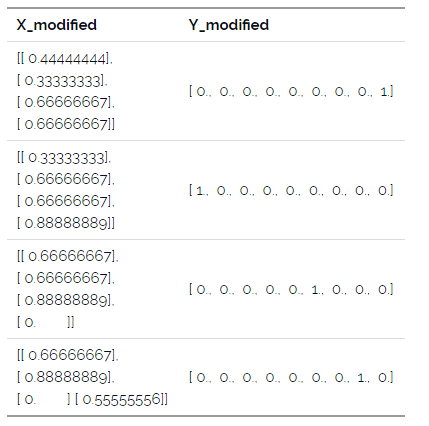
\includegraphics[width=0.6\linewidth,keepaspectratio]{rnn3}
%%%\end{center}
%%%\begin{itemize}
%%%\item SYNAPSE\_0 propagates the input data to the hidden layer. 
%%%\item SYNAPSE\_1 propagates the hidden layer to the output data. 
%%%\item The new matrix (SYNAPSE\_h, the recurrent one), propagates from the hidden layer (layer\_1) to the hidden layer at the next timestep (still layer\_1). 
%%%\end{itemize}
%%%\end{frame}

%%%%%%%%%%%%%%%%%%%%%%%%%%%%%%%%%%%%%%%%%%%%%%%%%%%
\begin{frame}[fragile] \frametitle{RNN - Summary}
\begin{center}
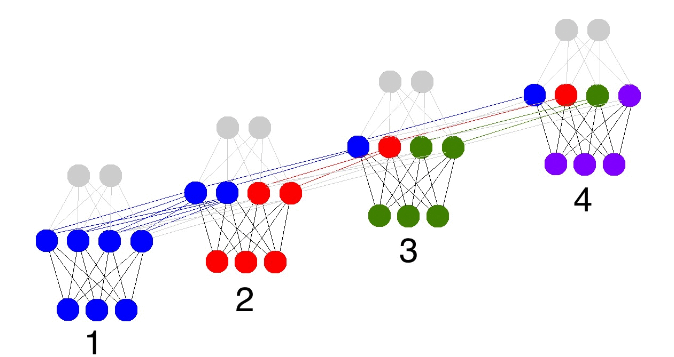
\includegraphics[width=0.6\linewidth,keepaspectratio]{rnn4}
\end{center}
\begin{itemize}
\item It depicts 4 timesteps. 
\item The first is exclusively influenced by the input data. 
\item The second one is a mixture of the first and second inputs. 
\item This continues on. 
\end{itemize}
\end{frame}

%%%%%%%%%%%%%%%%%%%%%%%%%%%%%%%%%%%%%%%%%%%%%%%%%%%
\begin{frame}[fragile] \frametitle{RNN - Summary}
\begin{center}
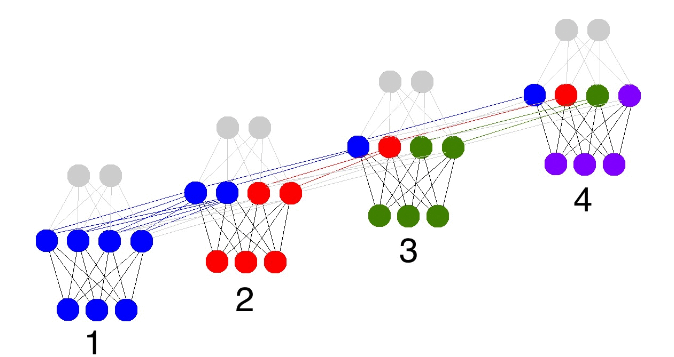
\includegraphics[width=0.6\linewidth,keepaspectratio]{rnn4}
\end{center}
\begin{itemize}
\item You should recognize that, in some way, network 4 is ''full''. 
\item Presumably, timestep 5 would have to choose which memories to keep and which ones to overwrite. 
\item It's the notion of memory ''capacity''. As you might expect, bigger layers can hold more memories for a longer period of time.
\end{itemize}
\end{frame}

%%%%%%%%%%%%%%%%%%%%%%%%%%%%%%%%%%%%%%%%%%%%%%%%%%%
\begin{frame}[fragile] \frametitle{RNN - Summary}
\begin{center}
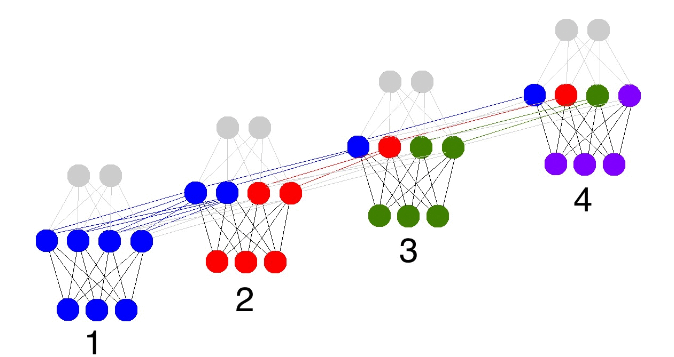
\includegraphics[width=0.6\linewidth,keepaspectratio]{rnn4}
\end{center}
\begin{itemize}
\item Also, this is when the network learns to forget irrelevant memories and remember important memories. 
\item What significant thing do you notice in timestep 3? 
\item Why is there more green in the hidden layer than the other colors?
\end{itemize}
\end{frame}

%%%%%%%%%%%%%%%%%%%%%%%%%%%%%%%%%%%%%%%%%%%%%%%%%%%
\begin{frame}[fragile] \frametitle{RNN - Summary}
\begin{itemize}
\item Also notice that the hidden layer is the barrier between the input and the output. 
\item In reality, the output is no longer a pure function of the input. 
\item The input is just changing what's in the memory, 
\item and the output is exclusively based on the memory. 
\end{itemize}
\end{frame}

%%%%%%%%%%%%%%%%%%%%%%%%%%%%%%%%%%%%%%%%%%%%%%%%%%%
\begin{frame}[fragile] \frametitle{RNN - Summary}
\begin{center}
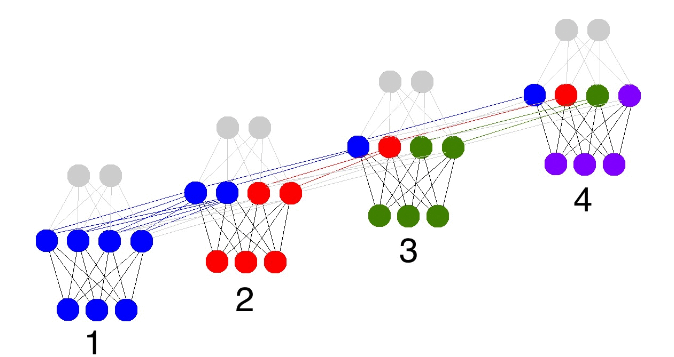
\includegraphics[width=0.6\linewidth,keepaspectratio]{rnn4}
\end{center}
\begin{itemize}
\item Another interesting takeaway. 
\item If there was no input at timesteps 2,3,and 4, the hidden layer would still change from timestep to timestep. 
\end{itemize}
\end{frame}

%%%%%%%%%%%%%%%%%%%%%%%%%%%%%%%%%%%%%%%%%%%%%%%%%%%
\begin{frame}[fragile] \frametitle{Back-propagation Through Time}
\begin{center}
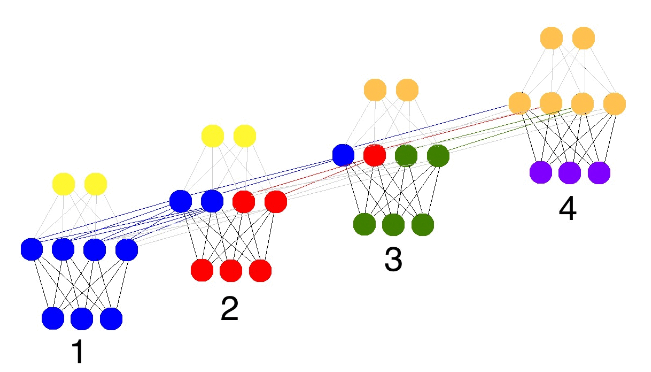
\includegraphics[width=0.6\linewidth,keepaspectratio]{rnn5}
\end{center}
\begin{itemize}
\item So, how do recurrent neural networks learn? 
\item Errors are bright yellow, derivatives are mustard colored.
\item Picture shows back propagation coming from 4th step upto 3rd.
\end{itemize}
\end{frame}

%%%%%%%%%%%%%%%%%%%%%%%%%%%%%%%%%%%%%%%%%%%%%%%%%%%
\begin{frame}[fragile] \frametitle{Back-propagation Through Time}
\begin{center}
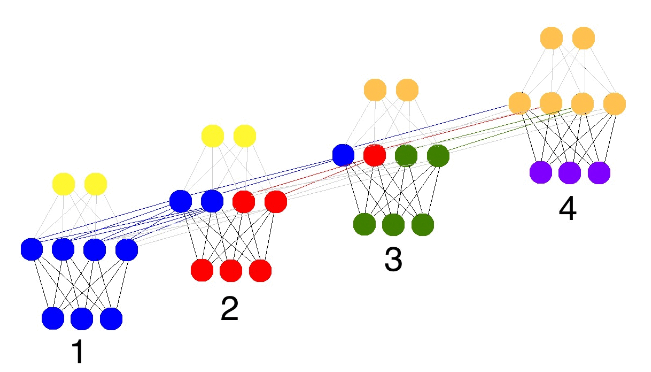
\includegraphics[width=0.6\linewidth,keepaspectratio]{rnn5}
\end{center}
\begin{itemize}
\item They learn by fully propagating forward from 1 to 4 and then back-propagating all the derivatives from 4 back to 1. 
\item Its normal neural network, except that we're re-using the same weights (synapses 0,1,and h) in their respective places. 
\end{itemize}
\end{frame}


%%%%%%%%%%%%%%%%%%%%%%%%%%%%%%%%%%%%%%%%%%%%%%%%%%%%%
%%\begin{frame}[fragile] \frametitle{Recurrent neural networks}
%%
%%\begin{itemize}
%%\item Recurrent Neural Networks are networks with loops in them, allowing information to persist.
%%\item In the above diagram, a chunk of neural network, A, looks at some input xt and outputs a value ht. 
%%\item A loop allows information to be passed from one step of the network to the next. 
%%\end{itemize}
%%\end{frame}



%%%%%%%%%%%%%%%%%%%%%%%%%%%%%%%%%%%%%%%%%%%%%%%%%%%
\begin{frame}[fragile] \frametitle{RNNs advantages}

\begin{itemize}
\item The applications of standard Neural Networks (and also Convolutional Networks) are limited due to:
\item They only accepted a fixed-size vector as input (e.g., an image) and produce a fixed-size vector as output (e.g., probabilities of different classes). 
\item These models use a fixed amount of computational steps (e.g. the number of layers in the model).
\end{itemize}
\end{frame}

%%%%%%%%%%%%%%%%%%%%%%%%%%%%%%%%%%%%%%%%%%%%%%%%%%%
\begin{frame}[fragile] \frametitle{RNNs advantages}

\begin{itemize}
\item Recurrent Neural Networks are unique as they allow us to operate over sequences of vectors.
\item Sequences in the input, the output, or in the most general case both
\end{itemize}
\end{frame}


%%%
%%%
%%%
%%%
%%%%%%%%%%%%%%%%%%%%%%%%%%%%%%%%%%%%%%%%%%%%%%%%%%%%%%
%%%\begin{frame}[fragile] \frametitle{Stateful models}
%%%
%%%
%%%\begin{itemize}
%%%\item Using this idea, we can think of variable width inputs
%%%such that each new word simply updates our current prediction.
%%%In this way an RNN has two types of data inside of it:
%%%\begin{itemize}
%%%\item fixed weights, just as we have been using with CNNs
%%%\item stateful variables that are updated as it observes words
%%%in a document
%%%\end{itemize}
%%%\item Can also think of this as giving `memory' to the neural
%%%network.
%%%\end{itemize}
%%%\end{frame}
%%%
%%%
%%%
%%%%%%%%%%%%%%%%%%%%%%%%%%%%%%%%%%%%%%%%%%%%%%%%%%%%%%
%%%\begin{frame}[fragile] \frametitle{RNNs Memory}
%%%\begin{center}
%%%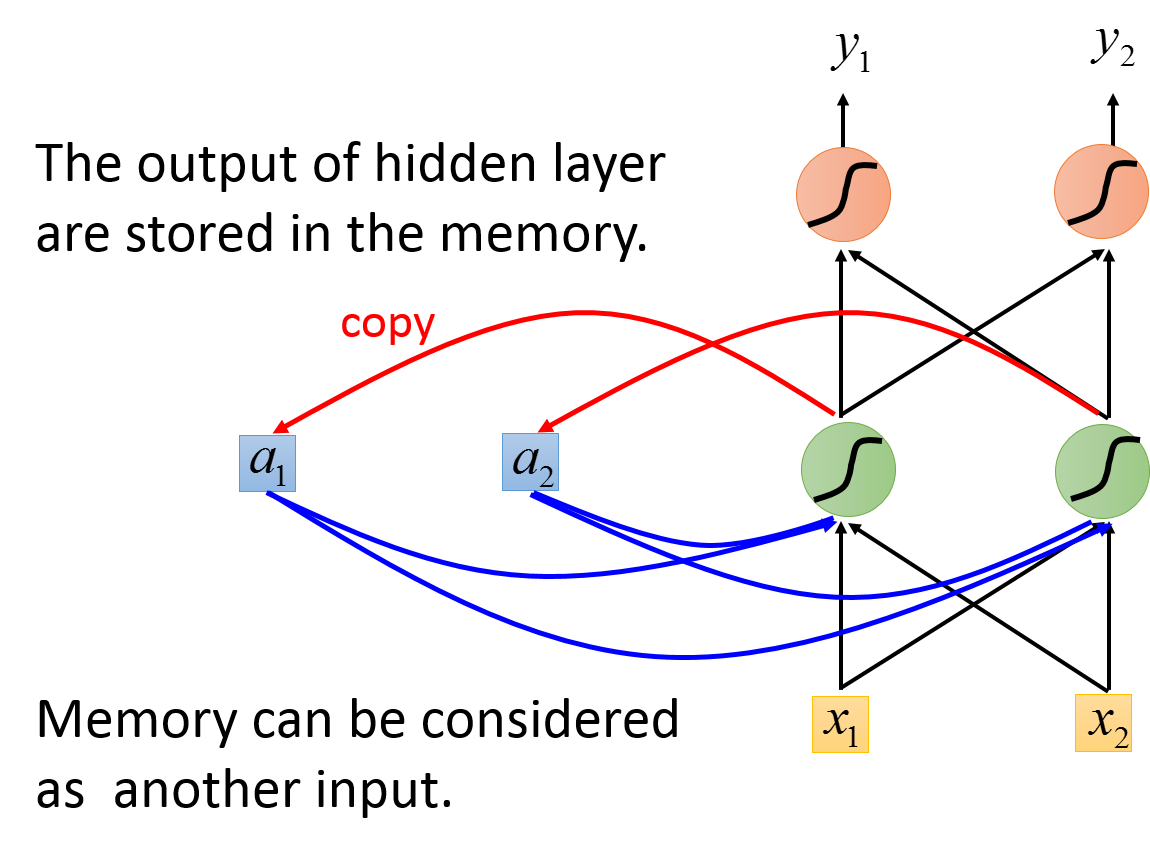
\includegraphics[width=0.8\linewidth,keepaspectratio]{rnnmem}
%%%\end{center}
%%%\end{frame}
%%%
%%%
%%%
%%%%%%%%%%%%%%%%%%%%%%%%%%%%%%%%%%%%%%%%%%%%%%%%%%%%%%
%%%\begin{frame}[fragile] \frametitle{}
%%%
%%%
%%%
%%%A third way of thinking about recurrent neural networks is to
%%%think of a network that has a loop in it. However, the self-input
%%%get's applied the \textit{next} time it is called.
%%%
%%%\begin{center}
%%%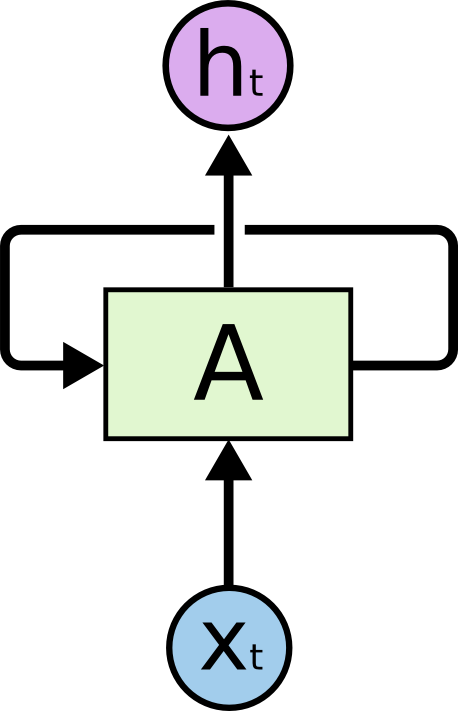
\includegraphics[width=0.3\linewidth,keepaspectratio]{cloah01.png}
%%%\end{center}
%%%
%%%\end{frame}
%%%
%%%%%%%%%%%%%%%%%%%%%%%%%%%%%%%%%%%%%%%%%%%%%%%%%%%%%%
%%%\begin{frame}[fragile] \frametitle{}
%%%
%%%A fourth way of thinking about a recurrent neural network is
%%%mathematically. We now have two parts to the update function
%%%in the RNN:
%%%\begin{align*}
%%%h_{t} &= {W x_t + b} + {U h_{t-1}}
%%%\end{align*}
%%%Notice that $U$ must always be a square matrix,
%%%because we could unravel this one time further to yield:
%%%\begin{align*}
%%%h_{t} &= W x_t + b + U W x_{t-1} + U b + U^2 h_{t-2}
%%%\end{align*}
%%%
%%%\end{frame}
%%%
%%%%%%%%%%%%%%%%%%%%%%%%%%%%%%%%%%%%%%%%%%%%%%%%%%%%%%
%%%\begin{frame}[fragile] \frametitle{What's different?}
%%%\begin{itemize}
%%%\item At each time step, output of hidden layers $H$ are added back for the next input.
%%%\item Outputs are also calculated at each time step ($Y_t$)
%%%\item Same wts and biases are shared across iterations
%%%\item Its like a state machine cell (remembering something)
%%%\item Can be used for sequences
%%%\end{itemize}
%%%
%%%
%%%\end{frame}
%%%
%%%%%%%%%%%%%%%%%%%%%%%%%%%%%%%%%%%%%%%%%%%%%%%%%%%%%%
%%%\begin{frame}[fragile] \frametitle{What's different?}
%%%\begin{center}
%%%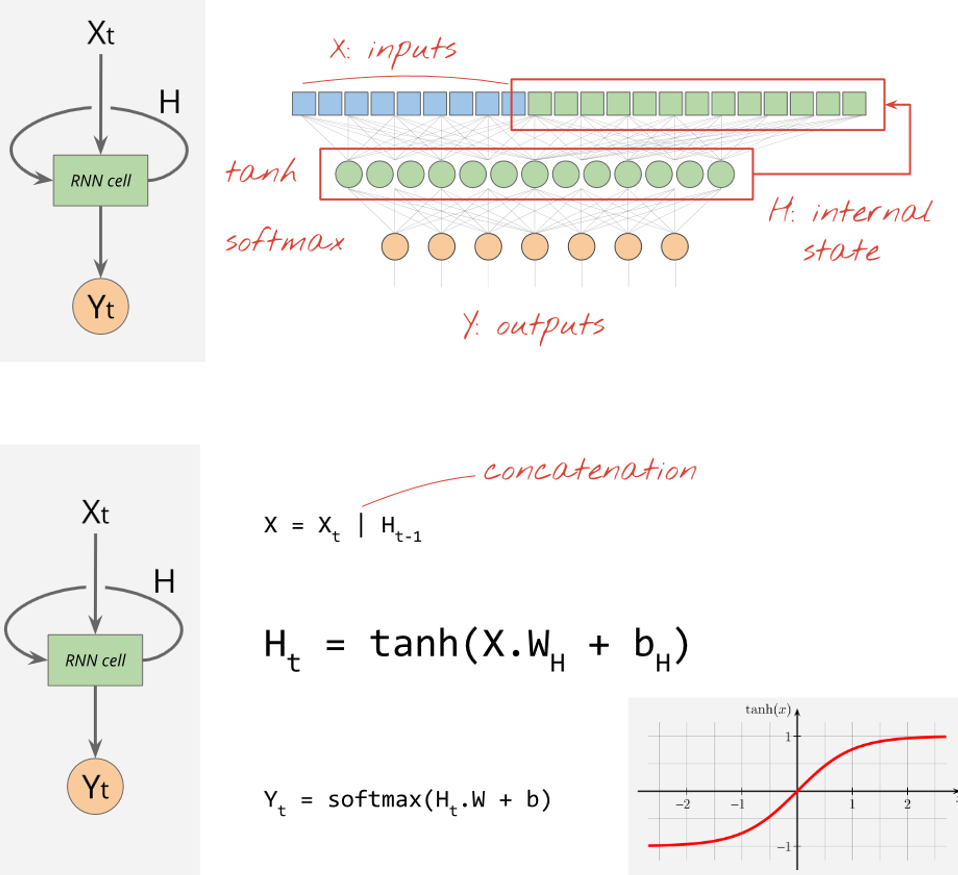
\includegraphics[width=0.8\linewidth,keepaspectratio]{rnnwts}
%%%\end{center}
%%%
%%%\end{frame}
%%%
%%%
%%%
%%%%%%%%%%%%%%%%%%%%%%%%%%%%%%%%%%%%%%%%%%%%%%%%%%%%%%
%%%\begin{frame}[fragile] \frametitle{RNN}
%%%
%%%\begin{center}
%%%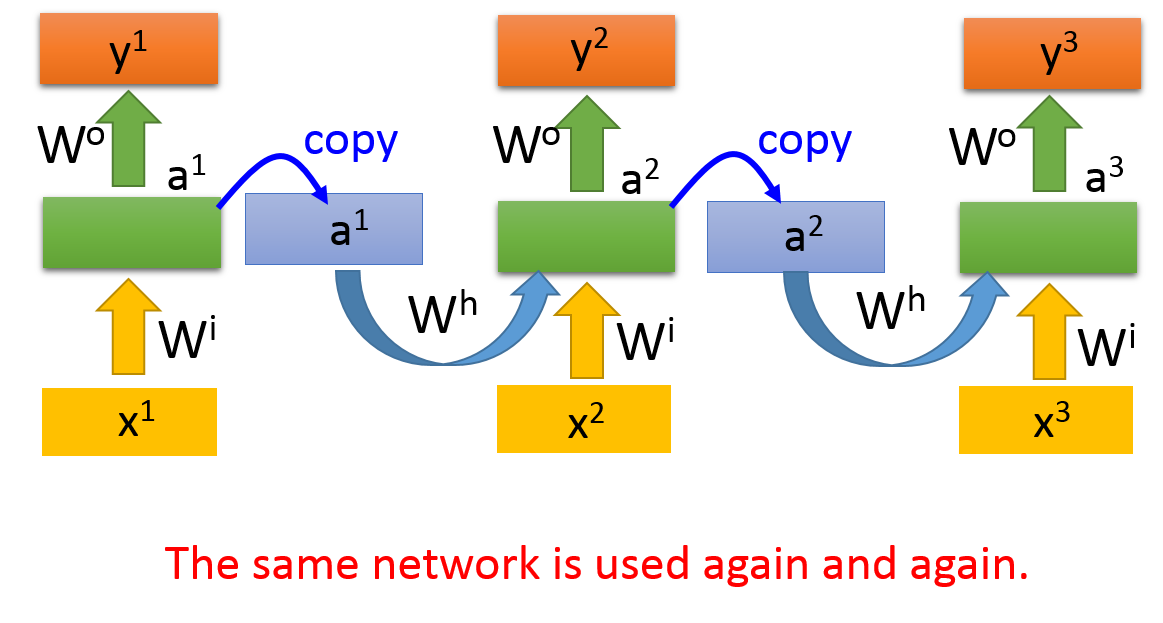
\includegraphics[width=0.8\linewidth,keepaspectratio]{rnnsamewts}
%%%\end{center}
%%%Output $y^i$ depends on $x_1, x_2,\ldots x_i$
%%%
%%%\end{frame}
%%%
%%%%%%%%%%%%%%%%%%%%%%%%%%%%%%%%%%%%%%%%%%%%%%%%%%%%%%
%%%\begin{frame}[fragile] \frametitle{On Sequences}
%%%
%%%
%%%\begin{itemize}
%%%\item Each cell, gets input, does iterations to try to match with given outputs. In the process, calculates wts and biases, as usual. May not work. 
%%%\item Instead of one cell, have a series and see if $Y_5$ can be forced.
%%%\item It is achieved by backpropagating through all cells, backwards.
%%%\item All $H$''s are adjusted, so $W$''s and $b$''s
%%%\item Can train on sequence of characters and verify open and close brackets
%%%\end{itemize}
%%%\begin{center}
%%%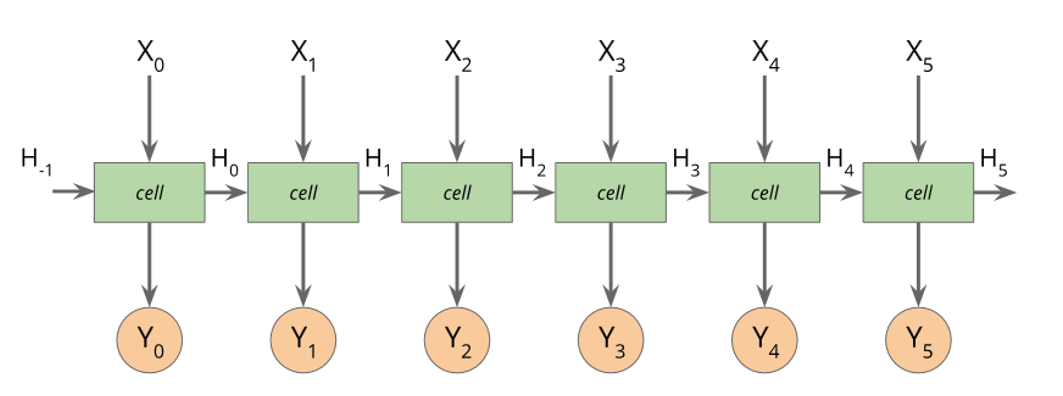
\includegraphics[width=0.8\linewidth,keepaspectratio]{rnnseq}
%%%\end{center}
%%%
%%%\end{frame}
%%%
%%%%%%%%%%%%%%%%%%%%%%%%%%%%%%%%%%%%%%%%%%%%%%%%%%%%%%
%%%\begin{frame}[fragile] \frametitle{How to train RNN?}
%%%
%%%\begin{center}
%%%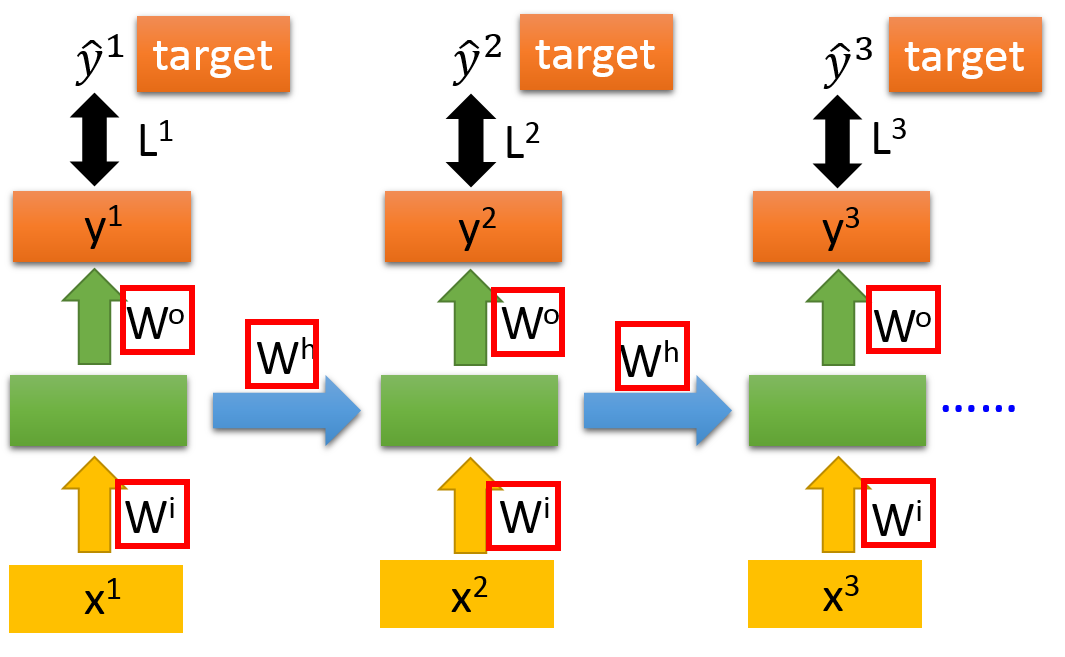
\includegraphics[width=0.8\linewidth,keepaspectratio]{rnntrain}
%%%\end{center}
%%%Find the network parameters to minimize the total cost
%%%
%%%\end{frame}
%%%
%%%
%%%
%%%%%%%%%%%%%%%%%%%%%%%%%%%%%%%%%%%%%%%%%%%%%%%%%%%%%%
%%%\begin{frame}[fragile] \frametitle{Of course it can be deep}
%%%\begin{center}
%%%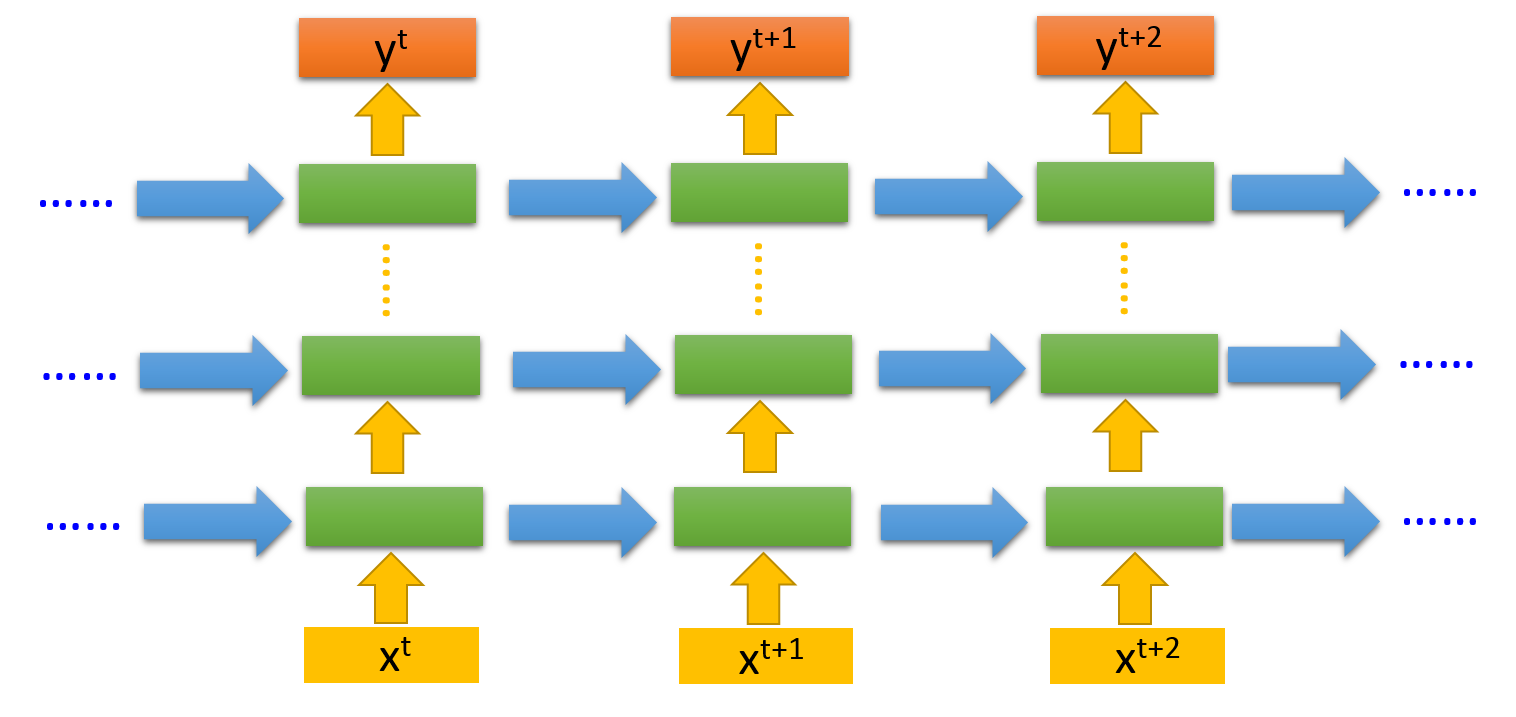
\includegraphics[width=0.8\linewidth,keepaspectratio]{rnndeep}
%%%\end{center}
%%%\end{frame}
%%%
%%%%%%%%%%%%%%%%%%%%%%%%%%%%%%%%%%%%%%%%%%%%%%%%%%%%%%
%%%\begin{frame}[fragile] \frametitle{Bidirectional RNN}
%%%\begin{center}
%%%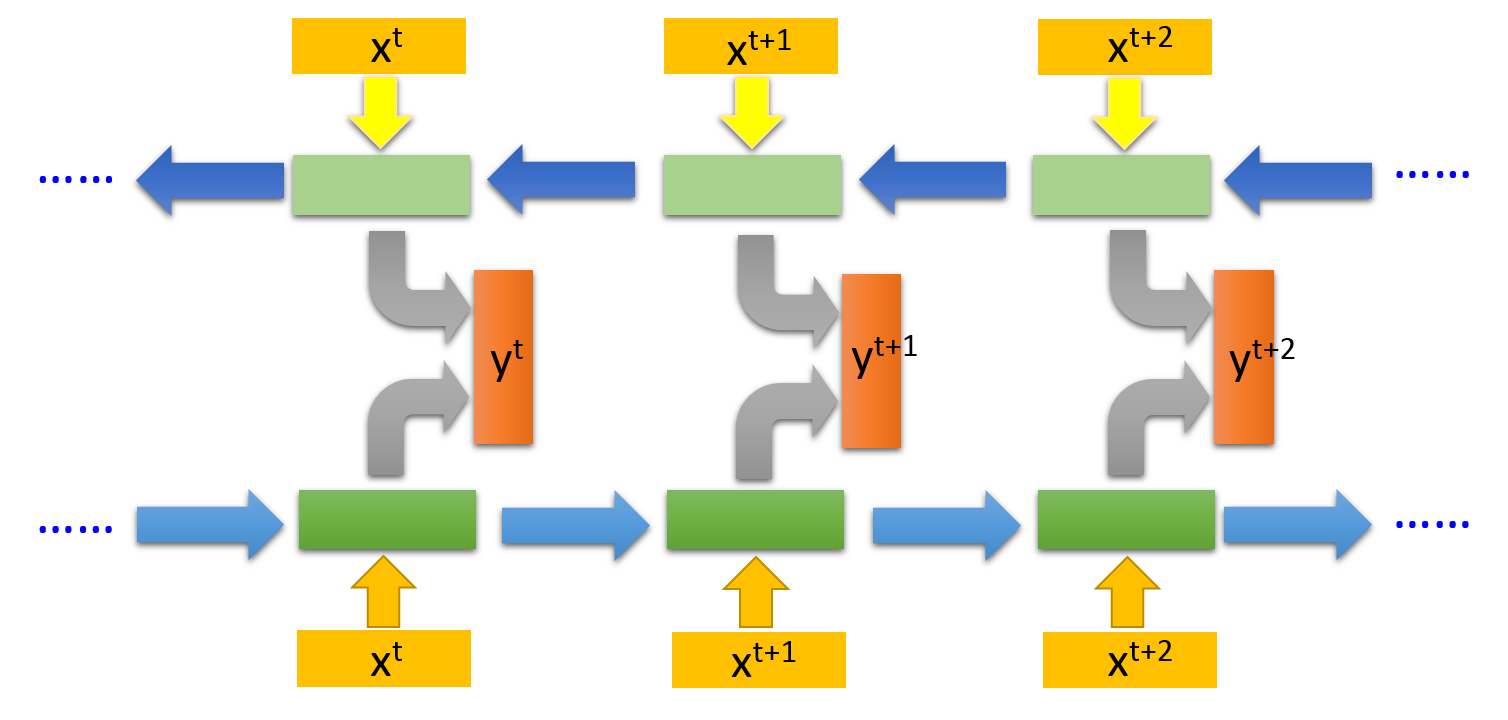
\includegraphics[width=\linewidth,keepaspectratio]{rnnbi}
%%%\end{center}
%%%\end{frame}
%%%
%%%%%%%%%%%%%%%%%%%%%%%%%%%%%%%%%%%%%%%%%%%%%%%%%%%%%%
%%%\begin{frame}[fragile] \frametitle{Bidirectional RNN}
%%%\begin{center}
%%%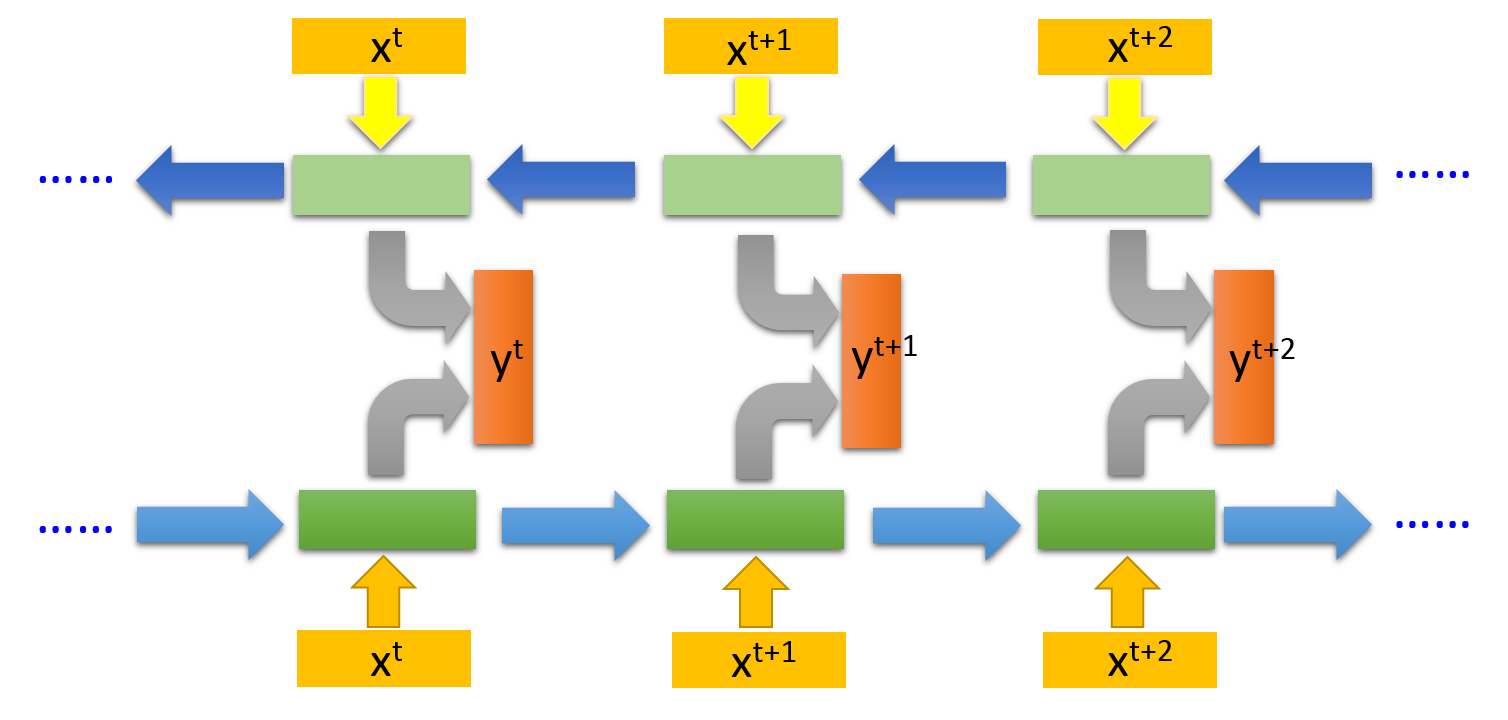
\includegraphics[width=\linewidth,keepaspectratio]{rnnbi}
%%%\end{center}
%%%\end{frame}
%%%
%%%
%%%%%%%%%%%%%%%%%%%%%%%%%%%%%%%%%%%%%%%%%%%%%%%%%%%%%%
%%%\begin{frame}[fragile] \frametitle{Many to Many (Output is shorter)}
%%%Both input and output are both sequences, but the output is shorter.
%%%E.g. Speech Recognition
%%%\begin{center}
%%%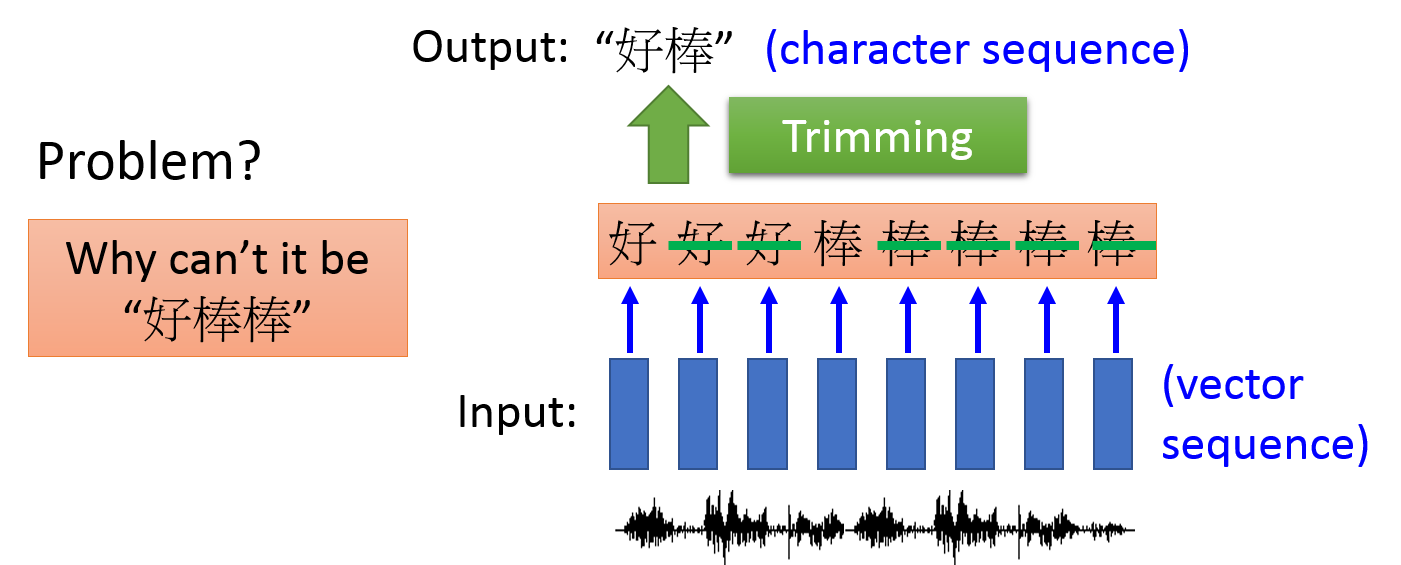
\includegraphics[width=\linewidth,keepaspectratio]{rnnmm}
%%%\end{center}
%%%\end{frame}
%%%
%%%%%%%%%%%%%%%%%%%%%%%%%%%%%%%%%%%%%%%%%%%%%%%%%%%%%%
%%%\begin{frame}[fragile] \frametitle{Can also Stack them}
%%%\begin{center}
%%%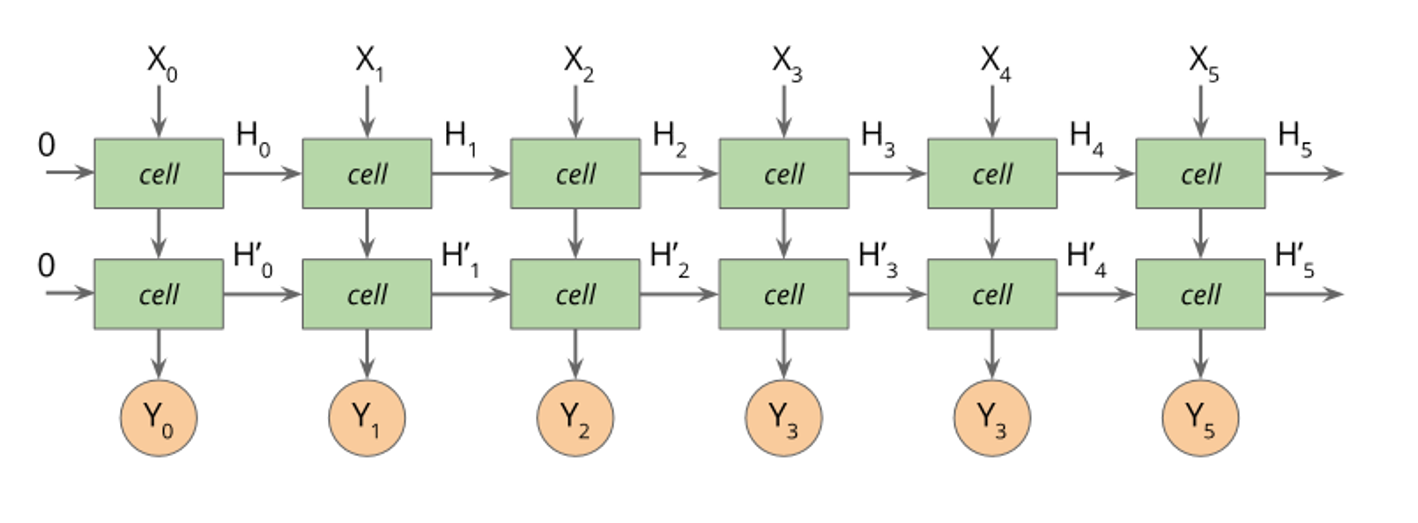
\includegraphics[width=\linewidth,keepaspectratio]{rnnstack}
%%%\end{center}
%%%\end{frame}
%%%
%%%%%%%%%%%%%%%%%%%%%%%%%%%%%%%%%%%%%%%%%%%%%%%%%%%%%%
%%%\begin{frame}[fragile] \frametitle{RNN Types a summary}
%%%Input vectors are in red, output vectors are in blue and green vectors hold the RNN's state
%%%\begin{center}
%%%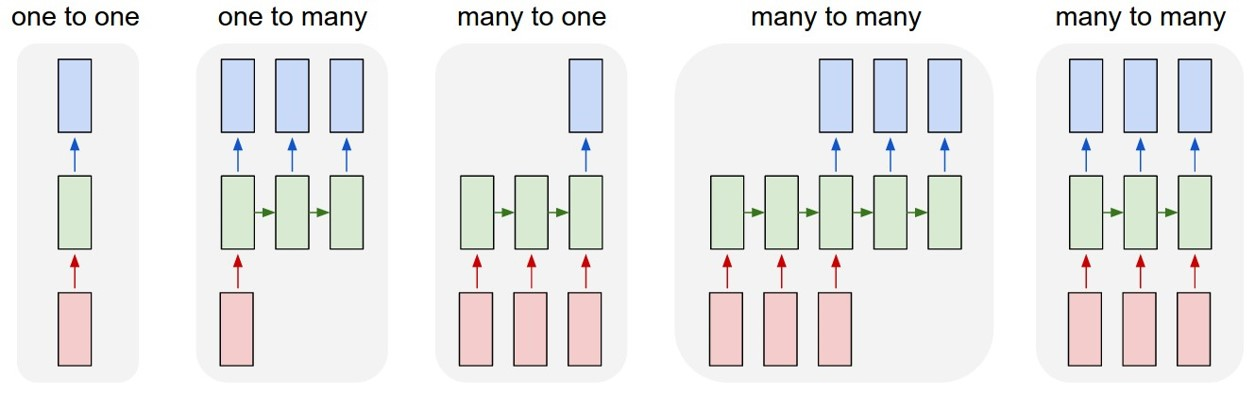
\includegraphics[width=\linewidth,keepaspectratio]{rnntypes}
%%%\end{center}
%%%
%%%\end{frame}
%%%
%%%%%%%%%%%%%%%%%%%%%%%%%%%%%%%%%%%%%%%%%%%%%%%%%%%%%%
%%%\begin{frame}[fragile] \frametitle{RNN Types a summary}
%%%\begin{itemize}
%%%\item Standard mode of processing without RNN, from fixed-sized input to fixed-sized output (e.g. image classification). 
%%%\item Sequence output (e.g. image captioning takes an image and outputs a sentence of words). 
%%%\item Sequence input (e.g. sentiment analysis where a given sentence is classified as expressing positive or negative sentiment). 
%%%\item Sequence input and sequence output (e.g. Machine Translation: an RNN reads a sentence in English and then outputs a sentence in French). 
%%%\item Synced sequence input and output (e.g. video classification where we wish to label each frame of the video).
%%%\end{itemize}
%%%\end{frame}
%%%
%%%%%%%%%%%%%%%%%%%%%%%%%%%%%%%%%%%%%%%%%%%%%%%%%%%%%%
%%%\begin{frame}[fragile] \frametitle{RNN Apps}
%%%\begin{center}
%%%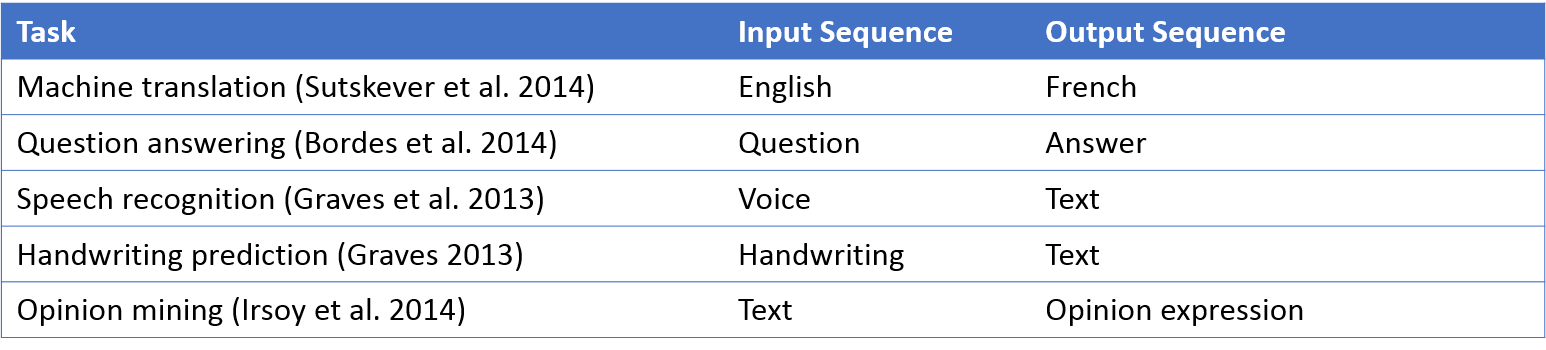
\includegraphics[width=\linewidth,keepaspectratio]{rnnapps}
%%%\end{center}
%%%\end{frame}
%%%
%%%%%%%%%%%%%%%%%%%%%%%%%%%%%%%%%%%%%%%%%%%%%%%%%%%%%%
%%%\begin{frame}[fragile] \frametitle{Name Entity Recognition}
%%%Detecting named entities like name of people, locations, organization, etc. in a sentence.
%%%\begin{center}
%%%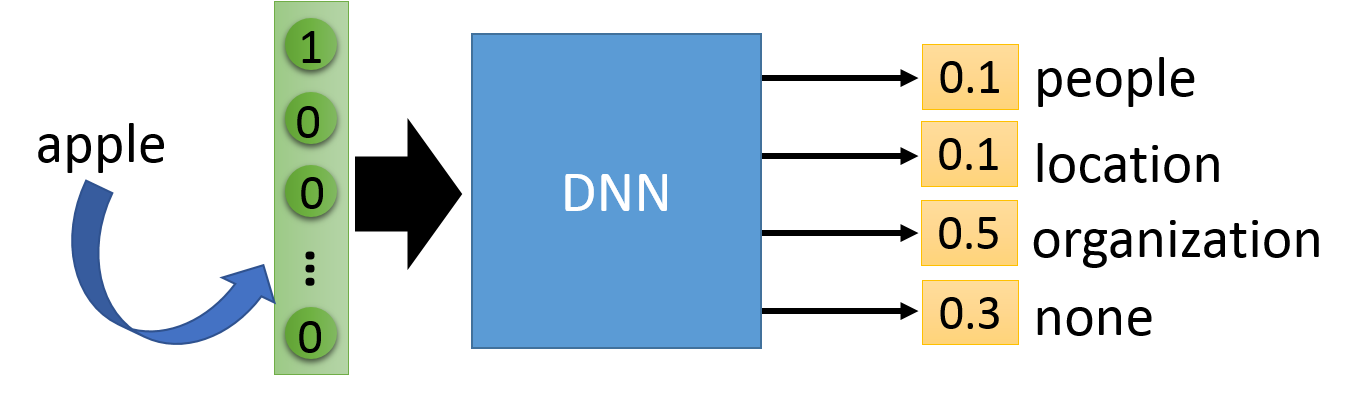
\includegraphics[width=\linewidth,keepaspectratio]{rnnner}
%%%\end{center}
%%%\end{frame}
%%%
%%%%%%%%%%%%%%%%%%%%%%%%%%%%%%%%%%%%%%%%%%%%%%%%%%%%%%
%%%\begin{frame}[fragile] \frametitle{Name Entity Recognition}
%%%\begin{center}
%%%\includegraphics[width=\linewidth,keepaspectratio]{rnnnerlayer}
%%%\end{center}
%%%\end{frame}
%%%
%%%%%%%%%%%%%%%%%%%%%%%%%%%%%%%%%%%%%%%%%%%%%%%%%%%%%%
%%%\begin{frame}[fragile] \frametitle{Unfortunately}
%%%RNN-based network is not always easy to learn
%%%\begin{center}
%%%\includegraphics[width=\linewidth,keepaspectratio]{rnndisadv}
%%%\end{center}
%%%\end{frame}
%%%
%%%%%%%%%%%%%%%%%%%%%%%%%%%%%%%%%%%%%%%%%%%%%%%%%%%%%%
%%%\begin{frame}[fragile] \frametitle{Errors}
%%%The error surface is rough.
%%%\begin{center}
%%%\includegraphics[width=\linewidth,keepaspectratio]{rnnerr}
%%%\end{center}
%%%\end{frame}
%%%
%%%
%%%%%%%%%%%%%%%%%%%%%%%%%%%%%%%%%%%%%%%%%%%%%%%%%%%%%%
%%%\begin{frame}[fragile] \frametitle{Anything better}
%%%\begin{itemize}
%%%\item ``Michael was born in Paris.<sentences> His mother tongue is ''
%%%\item Clue is far away. You need to have very long chain of such cells. That's limitation.
%%%\item Just few words is ok.
%%%\item Solution: LSTM (Long Short Term Memory)
%%%\end{itemize}
%%%\end{frame}
%%%
%%%
%%%%%%%%%%%%%%%%%%%%%%%%%%%%%%%%%%%%%%%%%%%%%%%%%%%%%%
%%%\begin{frame}[fragile] \frametitle{Anything better}
%%%\begin{center}
%%%\includegraphics[width=\linewidth,keepaspectratio]{rnn2lstm}
%%%\end{center}
%%%\end{frame}



%%%%%%%%%%%%%%%%%%%%%%%%%%%%%%%%%%%%%%%%%%%%%%%%%%%
\begin{frame}
  \begin{center}
    {\Large RNN variations}
    
    LSTM-GRU
  \end{center}
\end{frame}

%%%%%%%%%%%%%%%%%%%%%%%%%%%%%%%%%%%%%%%%%%%%%%%%%%%
\begin{frame}[fragile] \frametitle{Recap: Simple RNN}
\begin{center}
\includegraphics[width=0.5\linewidth,keepaspectratio]{lstm49}

\tiny{(Ref: Intro to Deep Learning - Coursera, National Research University Higher School of Economics)}
\end{center}
RNN takes previous hidden state ($h_{t-1}$), current input ($x_t$) and generates new/next hidden state ($h_t$) by formula $h_t = f_h ( Vx_t + Wh_{t-1} + b_h)$
\end{frame}

%%%%%%%%%%%%%%%%%%%%%%%%%%%%%%%%%%%%%%%%%%%%%%%%%%%
\begin{frame}[fragile] \frametitle{RNN Shortcomings}
\begin{itemize}
\item RNN does not work in some situations
\item Especially when long past words need to be accounted for
\item Due to Vanishing Gradient problem.
\end{itemize}
\end{frame}

%%%%%%%%%%%%%%%%%%%%%%%%%%%%%%%%%%%%%%%%%%%%%%%%%%%
\begin{frame}[fragile] \frametitle{Toy Example: RNN Shortcomings (Ref: Brandon Rohrer)}
Say we are writting a children's book, which has only 3 sentences
\begin{itemize}
\item ``Doug saw Jane.''
\item ``Jane saw Spot.''
\item ``Spot saw Doug.''
\item So the dictionary is : \{`Doug', `Jane', `Spot', `saw','.'\}, thats it.
\end{itemize}
\end{frame}

%%%%%%%%%%%%%%%%%%%%%%%%%%%%%%%%%%%%%%%%%%%%%%%%%%%
\begin{frame}[fragile] \frametitle{Toy Example: RNN Shortcomings}
\begin{itemize}
\item We are building a children's book
\item Meaning predicting next word, called ``language model''
\item Need to build neural network that will predict next probable word to generate good sentences.
\item We represent words as One-hot encoding, of size 5.
\item For `Doug', 1st position will be 1 rest all 0s. And so on.
\end{itemize}
\end{frame}

%%%%%%%%%%%%%%%%%%%%%%%%%%%%%%%%%%%%%%%%%%%%%%%%%%%
\begin{frame}[fragile] \frametitle{Toy Example: RNN Shortcomings}
Observations: Whenever we see names like `Doug', `Spot' or `Jane', most likely next word is `saw' or `.'
\begin{center}
\includegraphics[width=\linewidth,keepaspectratio]{lstm11}
\end{center}
\end{frame}

%%%%%%%%%%%%%%%%%%%%%%%%%%%%%%%%%%%%%%%%%%%%%%%%%%%
\begin{frame}[fragile] \frametitle{Toy Example: RNN Shortcomings}
Observations: If we had predicted a name in the previous time step, those will also vote for `saw' or `.'
\begin{center}
\includegraphics[width=0.8\linewidth,keepaspectratio]{lstm12}
\end{center}
\end{frame}

%%%%%%%%%%%%%%%%%%%%%%%%%%%%%%%%%%%%%%%%%%%%%%%%%%%
\begin{frame}[fragile] \frametitle{Toy Example: RNN Shortcomings}
Observations: Whenever we see names like `saw', or `.', most likely next word is amongst names.
\begin{center}
\includegraphics[width=0.8\linewidth,keepaspectratio]{lstm13}
\end{center}
\end{frame}


%%%%%%%%%%%%%%%%%%%%%%%%%%%%%%%%%%%%%%%%%%%%%%%%%%%
\begin{frame}[fragile] \frametitle{Toy Example: RNN Shortcomings}
\begin{itemize}
\item Inputs are shown by network symbol below
\item And the activation function is the sigmoid (makes to 0 to 1)
\end{itemize}
\begin{center}
\includegraphics[width=0.8\linewidth,keepaspectratio]{lstm14}
\end{center}
\end{frame}

%%%%%%%%%%%%%%%%%%%%%%%%%%%%%%%%%%%%%%%%%%%%%%%%%%%
\begin{frame}[fragile] \frametitle{Toy Example: RNN Shortcomings}
\begin{itemize}
\item But the problem is ``Doug saw'' can predict any name next, and it can be ``Doug'' again.
\item Thats a bad prediction, even though, by rules formed so far, it is correct.
\item Another mistake ``Jane saw Spot saw Doug saw \ldots''
\item This is because, we are seeing only one step behind.
\item To overcome this issue, we expand the RNN to accommodate Memory.
\item We want to be able to remember what happened many steps before.
\end{itemize}
\end{frame}


%%%%%%%%%%%%%%%%%%%%%%%%%%%%%%%%%%%%%%%%%%%%%%%%%%%
\begin{frame}[fragile] \frametitle{Toy Example: RNN Addressing shortcomings}
\begin{center}
\includegraphics[width=\linewidth,keepaspectratio]{lstm15}
\end{center}
\end{frame}


%%%%%%%%%%%%%%%%%%%%%%%%%%%%%%%%%%%%%%%%%%%%%%%%%%%
\begin{frame}[fragile] \frametitle{Toy Example: RNN Addressing shortcomings}
Note:
\begin{itemize}
\item Squashing with flat bottom:0 to 1 
\item Plus gate does element wise addition
\item Cross gate does element wise multiplication. It acts like a knob/gate which passes only some/all portions through.
\end{itemize}
\begin{center}
\includegraphics[width=0.6\linewidth,keepaspectratio]{lstm15}
\end{center}
\end{frame}

%%%%%%%%%%%%%%%%%%%%%%%%%%%%%%%%%%%%%%%%%%%%%%%%%%%
\begin{frame}[fragile] \frametitle{Toy Example: RNN Addressing shortcomings}
\begin{itemize}
\item We still have previous output along with current input going as input to Neural network at the bottom, then full squashing.
\item Predictions from there get passed through.
\end{itemize}
\begin{center}
\includegraphics[width=0.8\linewidth,keepaspectratio]{lstm16}
\end{center}
\end{frame}

%%%%%%%%%%%%%%%%%%%%%%%%%%%%%%%%%%%%%%%%%%%%%%%%%%%
\begin{frame}[fragile] \frametitle{Toy Example: RNN Addressing shortcomings}
\begin{itemize}
\item A copy of those predictions is hold on to for the next time step.
\item Some of that (due to Cross gate), along with input from flat bottom squash are passed through. 
\item Gets added to predictions as Memories.
\end{itemize}
\begin{center}
\includegraphics[width=0.8\linewidth,keepaspectratio]{lstm16}
\end{center}
\end{frame}

%%%%%%%%%%%%%%%%%%%%%%%%%%%%%%%%%%%%%%%%%%%%%%%%%%%
\begin{frame}[fragile] \frametitle{Toy Example: RNN Addressing shortcomings}
\begin{itemize}
\item The NN in the middle is doing something else.
\item It learns to select to forget WHAT, remember WHAT. 
\item So, called as FORGETTING Gate.
\end{itemize}
\begin{center}
\includegraphics[width=0.8\linewidth,keepaspectratio]{lstm16}
\end{center}
\end{frame}


%%%%%%%%%%%%%%%%%%%%%%%%%%%%%%%%%%%%%%%%%%%%%%%%%%%
\begin{frame}[fragile] \frametitle{Toy Example: RNN Addressing shortcomings}
\begin{itemize}
\item One more NN gets added at the top, called SELECTION
\item We may not want to release all those memories now.
\item It has own NN, own voting process, to decide what should be kept internal and what should be released as prediction.
\end{itemize}
\begin{center}
\includegraphics[width=0.8\linewidth,keepaspectratio]{lstm17}
\end{center}
\end{frame}

%%%%%%%%%%%%%%%%%%%%%%%%%%%%%%%%%%%%%%%%%%%%%%%%%%%
\begin{frame}[fragile] \frametitle{Toy Example: RNN Addressing shortcomings}
\begin{itemize}
\item Also introduced a full squashing function on vertical path
\item Due to previous PLUS gate, things could be greater than one, so as to bring them back to -1 to 1 range.
\end{itemize}
\begin{center}
\includegraphics[width=0.8\linewidth,keepaspectratio]{lstm17}
\end{center}
\end{frame}

%%%%%%%%%%%%%%%%%%%%%%%%%%%%%%%%%%%%%%%%%%%%%%%%%%%
\begin{frame}[fragile] \frametitle{Toy Example: RNN Addressing shortcomings}
\begin{itemize}
\item One more NN, the IGNORING gate is also added
\item Ignores some of the  possibilities. 
\item Called ATTENTION mechanism.
\item The whole thing is now LSTM: Long Short Term Memory
\end{itemize}
\begin{center}
\includegraphics[width=0.8\linewidth,keepaspectratio]{lstm18}
\end{center}
\end{frame}

%%%%%%%%%%%%%%%%%%%%%%%%%%%%%%%%%%%%%%%%%%%%%%%%%%%
\begin{frame}[fragile] \frametitle{Toy Example: LSTM}
\begin{itemize}
\item All NNs start with random values
\item They learn the weights during training.
\end{itemize}
\begin{center}
\includegraphics[width=0.8\linewidth,keepaspectratio]{lstm18}
\end{center}
\end{frame}

%%%%%%%%%%%%%%%%%%%%%%%%%%%%%%%%%%%%%%%%%%%%%%%%%%%
\begin{frame}[fragile] \frametitle{Toy Example: LSTM walk-through}
\begin{itemize}
\item Lets assume that LSTM has been trained with the three sentences.
\item Now ``Doug'' is the most recent word
\end{itemize}
\begin{center}
\includegraphics[width=0.8\linewidth,keepaspectratio]{lstm19}
\end{center}
\end{frame}

%%%%%%%%%%%%%%%%%%%%%%%%%%%%%%%%%%%%%%%%%%%%%%%%%%%
\begin{frame}[fragile] \frametitle{Toy Example: LSTM walk-through}
\begin{itemize}
\item Lets assume that LSTM has been trained with the three sentences.
\item Now ``Doug'' is the most recent word
\end{itemize}
\begin{center}
\includegraphics[width=0.8\linewidth,keepaspectratio]{lstm19}
\end{center}
\end{frame}


%%%%%%%%%%%%%%%%%%%%%%%%%%%%%%%%%%%%%%%%%%%%%%%%%%%
\begin{frame}[fragile] \frametitle{Toy Example: LSTM walk-through}
\begin{itemize}
\item  Previously we had `.' and thus possible predictions were `Doug', `Jane' and `Spot'.
\item So, New information ``Doug''
\item Previous Predictions: `Doug', `Jane' and `Spot'.
\item We pass these two vectors are inputs.
\end{itemize}
\begin{center}
\includegraphics[width=0.8\linewidth,keepaspectratio]{lstm20}
\end{center}
\end{frame}

%%%%%%%%%%%%%%%%%%%%%%%%%%%%%%%%%%%%%%%%%%%%%%%%%%%
\begin{frame}[fragile] \frametitle{Toy Example: LSTM walk-through}
\begin{itemize}
\item  Previously we had `.' and thus possible predictions were `Doug', `Jane' and `Spot'.
\item So, New information ``Doug''
\item Previous Predictions: `Doug', `Jane' and `Spot'.
\end{itemize}
\begin{center}
\includegraphics[width=0.8\linewidth,keepaspectratio]{lstm20}
\end{center}
\end{frame}

%%%%%%%%%%%%%%%%%%%%%%%%%%%%%%%%%%%%%%%%%%%%%%%%%%%
\begin{frame}[fragile] \frametitle{Toy Example: LSTM walk-through}
\begin{itemize}
\item We pass these two vectors are inputs to all 4 NNs
\item They are learning to do: PREDICTION, IGNORING, FORGETTING, SELECTION.
\end{itemize}
\begin{center}
\includegraphics[width=0.8\linewidth,keepaspectratio]{lstm20}
\end{center}
\end{frame}

%%%%%%%%%%%%%%%%%%%%%%%%%%%%%%%%%%%%%%%%%%%%%%%%%%%
\begin{frame}[fragile] \frametitle{Toy Example: LSTM walk-through}
\begin{itemize}
\item First one makes positive prediction: `saw'
\item Having seen `Doug' it says negative prediction about `Doug' now. (HOW?? whats negative prediction? negative probability???, how??, because of full-activation??)
\end{itemize}
\begin{center}
\includegraphics[width=0.8\linewidth,keepaspectratio]{lstm21}
\end{center}
\end{frame}

%%%%%%%%%%%%%%%%%%%%%%%%%%%%%%%%%%%%%%%%%%%%%%%%%%%
\begin{frame}[fragile] \frametitle{Toy Example: LSTM walk-through}
\begin{itemize}
\item For this simple example, we need not look at ATTENTION so skipping IGNORING
\item Positive `saw' and negative `Doug' are passed forward.
\item Lets say, for now, there is no memory as well. So, passed forward.
\end{itemize}
\begin{center}
\includegraphics[width=0.8\linewidth,keepaspectratio]{lstm22}
\end{center}
\end{frame}

%%%%%%%%%%%%%%%%%%%%%%%%%%%%%%%%%%%%%%%%%%%%%%%%%%%
\begin{frame}[fragile] \frametitle{Toy Example: LSTM walk-through}
\begin{itemize}
\item SELECTION: As recent word was name, the next one has to be `saw' or `.'
\item So, block anything else, but allows only `saw', as prediction of the time step.
\end{itemize}
\begin{center}
\includegraphics[width=0.8\linewidth,keepaspectratio]{lstm23}
\end{center}
\end{frame}

%%%%%%%%%%%%%%%%%%%%%%%%%%%%%%%%%%%%%%%%%%%%%%%%%%%
\begin{frame}[fragile] \frametitle{Toy Example: LSTM walk-through}
Next time step
\begin{itemize}
\item Most recent prediction: `saw'
\item Next new information/word: `saw'.
\item So prediction is names: `Doug', `Jane' and `Spot'.
\end{itemize}
\begin{center}
\includegraphics[width=0.8\linewidth,keepaspectratio]{lstm24}
\end{center}
\end{frame}

%%%%%%%%%%%%%%%%%%%%%%%%%%%%%%%%%%%%%%%%%%%%%%%%%%%
\begin{frame}[fragile] \frametitle{Toy Example: LSTM walk-through}
\begin{itemize}
\item Skip IGNORING for now.
\item Positive `saw' and Negative `Doug' was stored in Memory at FORGETTING gate.
\item Forgets `saw' and allows negative `Doug' to go through, as logical next prediction.
\end{itemize}
\begin{center}
\includegraphics[width=0.8\linewidth,keepaspectratio]{lstm25}
\end{center}
\end{frame}

%%%%%%%%%%%%%%%%%%%%%%%%%%%%%%%%%%%%%%%%%%%%%%%%%%%
\begin{frame}[fragile] \frametitle{Toy Example: LSTM walk-through}
\begin{itemize}
\item At the PLUS gate, negative `Doug' and Positive `Doug' cancel.
\item This lets only `Jane' and `Spot' to go through.
\end{itemize}
\begin{center}
\includegraphics[width=0.8\linewidth,keepaspectratio]{lstm26}
\end{center}
\end{frame}


%%%%%%%%%%%%%%%%%%%%%%%%%%%%%%%%%%%%%%%%%%%%%%%%%%%
\begin{frame}[fragile] \frametitle{Toy Example: LSTM walk-through}
\begin{itemize}
\item SELECTION: knows that `saw' just occurred. Based on experience, names will happen next.
\item We now have predictions for only `Jane' and `Spot'.
\item This avoids repetition of `Doug' in the same sentence.
\item Thus, LSTM can look back couple of time steps.
\end{itemize}
\begin{center}
\includegraphics[width=0.8\linewidth,keepaspectratio]{lstm27}
\end{center}
\end{frame}



%%%%%%%%%%%%%%%%%%%%%%%%%%%%%%%%%%%%%%%%%%%%%%%%%%%
\begin{frame}[fragile] \frametitle{Why - LSTM}
Designed to overcome:
\begin{itemize}
\item Long-term dependencies
\item Vanishing/exploding gradients
\end{itemize}
We don't want  to remember  everything,  just  the  important  things  for a long time
\end{frame}

%%%%%%%%%%%%%%%%%%%%%%%%%%%%%%%%%%%%%%%%%%%%%%%%%%%
\begin{frame}[fragile] \frametitle{Recap: Simple LSTM}
\begin{center}
\includegraphics[width=0.5\linewidth,keepaspectratio]{lstm50}

\tiny{(Ref: Intro to Deep Learning - Coursera, National Research University Higher School of Economics)}
\end{center}
LSTM has two channels, the usual RNN channel like previous hidden state ($h_{t-1}$), current input ($x_t$) and new/next hidden state ($h_t$) and the second one of memory $c_t$ incoming and $c_{t-1}$ outgoing. Intermediate output $g$ is computed as $g_t = \hat{f} ( V_gx_t + W_gh_{t-1} + b_g)$
\end{frame}

%%%%%%%%%%%%%%%%%%%%%%%%%%%%%%%%%%%%%%%%%%%%%%%%%%%
\begin{frame}[fragile] \frametitle{Recap: Simple LSTM}
\begin{center}
\includegraphics[width=0.5\linewidth,keepaspectratio]{lstm50}

\tiny{(Ref: Intro to Deep Learning - Coursera, National Research University Higher School of Economics)}
\end{center}
LSTM has two controllers of this intermediate $g$ output. Input Gate and Output Gate (both give out outputs of same dimmension as hidden unit).
\end{frame}

%%%%%%%%%%%%%%%%%%%%%%%%%%%%%%%%%%%%%%%%%%%%%%%%%%%
\begin{frame}[fragile] \frametitle{Recap: Simple LSTM}
\begin{center}
\includegraphics[width=0.5\linewidth,keepaspectratio]{lstm52}

\tiny{(Ref: Intro to Deep Learning - Coursera, National Research University Higher School of Economics)}
\end{center}
Memory is added with dot product of input gate $i$ and $g$.
\end{frame}

%%%%%%%%%%%%%%%%%%%%%%%%%%%%%%%%%%%%%%%%%%%%%%%%%%%
\begin{frame}[fragile] \frametitle{Recap: Simple LSTM}
\begin{center}
\includegraphics[width=0.5\linewidth,keepaspectratio]{lstm53}

\tiny{(Ref: Intro to Deep Learning - Coursera, National Research University Higher School of Economics)}
\end{center}
Output gate $o$ controls what to read from memory and passed as next output/hidden state.
\end{frame}

%%%%%%%%%%%%%%%%%%%%%%%%%%%%%%%%%%%%%%%%%%%%%%%%%%%
\begin{frame}[fragile] \frametitle{Recap: Simple LSTM}
\begin{center}
\includegraphics[width=0.5\linewidth,keepaspectratio]{lstm54}

\tiny{(Ref: Intro to Deep Learning - Coursera, National Research University Higher School of Economics)}
\end{center}
As now, we have a short way (in form of memory) which has no sigmoid or gradient applied to it, so information decay (by vaniishing gradient) does not happen.
\end{frame}

%%%%%%%%%%%%%%%%%%%%%%%%%%%%%%%%%%%%%%%%%%%%%%%%%%%
\begin{frame}[fragile] \frametitle{Recap: Simple LSTM}
\begin{center}
\includegraphics[width=0.5\linewidth,keepaspectratio]{lstm55}

\tiny{(Ref: Intro to Deep Learning - Coursera, National Research University Higher School of Economics)}
\end{center}
Need to forget something at times, thats Forget Gate.
\end{frame}
%%%%%%%%%%%%%%%%%%%%%%%%%%%%%%%%%%%%%%%%%%%%%%%%%%%
\begin{frame}[fragile] \frametitle{Vanishing Gradient}
\begin{center}
\includegraphics[width=\linewidth,keepaspectratio]{lstm1}
\end{center}
\end{frame}

%%%%%%%%%%%%%%%%%%%%%%%%%%%%%%%%%%%%%%%%%%%%%%%%%%%
\begin{frame}[fragile] \frametitle{Why - Long-Term Dependencies}
\begin{center}
\includegraphics[width=\linewidth,keepaspectratio]{lstm2}
\end{center}
\end{frame}

%%%%%%%%%%%%%%%%%%%%%%%%%%%%%%%%%%%%%%%%%%%%%%%%%%%
\begin{frame}[fragile] \frametitle{Vanishing Gradients}

Discovered by Sepp Hochreiter and Yoshua Bengio

\begin{center}
\includegraphics[width=0.45\linewidth,keepaspectratio]{lstm30}
\includegraphics[width=0.45\linewidth,keepaspectratio]{lstm31}

\tiny{(Ref: Deep Learning A-Z - Kirill Eremenko)}
\end{center}


\end{frame}

%%%%%%%%%%%%%%%%%%%%%%%%%%%%%%%%%%%%%%%%%%%%%%%%%%%
\begin{frame}[fragile] \frametitle{Vanishing Gradients}

Gradient descent minimizes loss (C) to arrive at the best weight (thus $\hat{y}$)

\begin{center}
\includegraphics[width=0.8\linewidth,keepaspectratio]{lstm32}


\tiny{(Ref: Deep Learning A-Z - Kirill Eremenko)}
\end{center}

Weights are then updated in the back-propagation.

\end{frame}

%%%%%%%%%%%%%%%%%%%%%%%%%%%%%%%%%%%%%%%%%%%%%%%%%%%
\begin{frame}[fragile] \frametitle{Vanishing Gradients}

In RNN, information travels through time. In the figure below, each circle is not a node, but the whole layer.
During training, at each time step you can calculate error ($\epsilon$)

\begin{center}
\includegraphics[width=0.8\linewidth,keepaspectratio]{lstm33}


\tiny{(Ref: Deep Learning A-Z - Kirill Eremenko)}
\end{center}

\end{frame}

%%%%%%%%%%%%%%%%%%%%%%%%%%%%%%%%%%%%%%%%%%%%%%%%%%%
\begin{frame}[fragile] \frametitle{Vanishing Gradients}

Lets look at one single time step. Error is $\epsilon_t$. All the weights, not just below, but all (say, 50) the previous weights need to be updated. In forward pass $W_{rec}$ (Weight recurring) was the weight that was getting multiplied to output at each time step.
\begin{center}
\includegraphics[width=\linewidth,keepaspectratio]{lstm34}

\tiny{(Ref: Deep Learning A-Z - Kirill Eremenko)}
\end{center}

\end{frame}

%%%%%%%%%%%%%%%%%%%%%%%%%%%%%%%%%%%%%%%%%%%%%%%%%%%
\begin{frame}[fragile] \frametitle{Vanishing Gradients}
So in back-propogration, similar weight will again multiply to arrive at the previous steps. If $W_{rec}$ is small, values of gradient decrease rapidly (green arrows). Lower the gradient, updating weights ceases shortly. Rest of the network  does not get trained. 
\begin{center}
\includegraphics[width=\linewidth,keepaspectratio]{lstm34}

\tiny{(Ref: Deep Learning A-Z - Kirill Eremenko)}
\end{center}

\end{frame}


%%%%%%%%%%%%%%%%%%%%%%%%%%%%%%%%%%%%%%%%%%%%%%%%%%%
\begin{frame}[fragile] \frametitle{Vanishing Gradients}
So if $W_{rec}$ is small, you have Vanishing Gradient problem, else Exploding Gradient problem. It needs to  be 1.
\begin{center}
\includegraphics[width=\linewidth,keepaspectratio]{lstm34}

\tiny{(Ref: Deep Learning A-Z - Kirill Eremenko)}
\end{center}

\end{frame}


%%%%%%%%%%%%%%%%%%%%%%%%%%%%%%%%%%%%%%%%%%%%%%%%%%%
\begin{frame}[fragile] \frametitle{Summary: Vanishing Gradient}
When weight  or activation  functions  (their  derivatives)  are:
\begin{itemize}
\item $< 1$ Vanishing Gradients
\item $> 1$ Exploding Gradients
\end{itemize}
\begin{center}
\includegraphics[width=\linewidth,keepaspectratio]{lstm3}
\end{center}
\end{frame}

%%%%%%%%%%%%%%%%%%%%%%%%%%%%%%%%%%%%%%%%%%%%%%%%%%%
\begin{frame}[fragile] \frametitle{Vanishing Gradients: Solutions}
Exploding Gradient:
\begin{itemize}
\item Truncating back-propagation
\item Penalties
\item Gradient Clipping
\end{itemize}
Vanishing Gradient:
\begin{itemize}
\item Weight Initialization
\item Echo State Networks
\item LSTM \ldots
\end{itemize}

\end{frame}




%%%%%%%%%%%%%%%%%%%%%%%%%%%%%%%%%%%%%%%%%%%%%%%%%%%
\begin{frame}[fragile] \frametitle{Vanishing Gradients: Solution: LSTM}
One solution could be to have  $W_{rec} = 1$. Gets rid off the problem.
Discovered by Sepp and Jurgen (his supervisor)
\begin{center}
\includegraphics[width=\linewidth,keepaspectratio]{lstm35}

\tiny{(Ref: Deep Learning A-Z - Kirill Eremenko)}
\end{center}

\end{frame}




%%%%%%%%%%%%%%%%%%%%%%%%%%%%%%%%%%%%%%%%%%%%%%%%%%%
\begin{frame}[fragile] \frametitle{LSTM}
\begin{itemize}
\item LSTM is the most sensible RNN architecture (ref: reddit)
\item It can be derived directly from RNN in 2 steps
\begin{itemize}
\item Don't multiply, use Addition instead
\item Gate all operations so that you don't cram everything
\end{itemize}
\end{itemize}
\end{frame}

%%%%%%%%%%%%%%%%%%%%%%%%%%%%%%%%%%%%%%%%%%%%%%%%%%%
\begin{frame}[fragile] \frametitle{Why - Don't multiply}
\begin{itemize}
\item Means, instead of multiplying the previous hidden state by a matrix to get the new state, you add something to your old hidden state and get the new state (here its not called as ``hidden'' but ``cell'')
\item Why?
\item Because, Multiplication == Vanishing Gradients.
\end{itemize}
\end{frame}

%%%%%%%%%%%%%%%%%%%%%%%%%%%%%%%%%%%%%%%%%%%%%%%%%%%
\begin{frame}[fragile] \frametitle{Why - Gate all operations}
\begin{itemize}
\item Now we are capable of long term memory since we are not losing it by repeated multiplications.
\item But is storing everything useful?
\item Also, do we want to output everything we have stored at each instant.
\item NO.
\end{itemize}
\end{frame}

%%%%%%%%%%%%%%%%%%%%%%%%%%%%%%%%%%%%%%%%%%%%%%%%%%%
\begin{frame}[fragile] \frametitle{Why - Gate all operations}
\begin{itemize}
\item There are 3 steps in RNN: input to hidden, hidden to hidden, hidden to output
\item LSTM regulates each with input, forget and output gates respectively.
\item Each of the gates are calculated as function of what we already know (ie previous) and the current input
\item Now our internal hidden state will becomes holy and restricted. So, its called as ``Cell''.
\end{itemize}
\end{frame}


%%%%%%%%%%%%%%%%%%%%%%%%%%%%%%%%%%%%%%%%%%%%%%%%%%%
\begin{frame}[fragile] \frametitle{LSTM Architecture}
\begin{center}
\includegraphics[width=\linewidth,keepaspectratio]{lstm36}

\tiny{(Ref: Deep Learning A-Z - Kirill Eremenko, Original Chris Olah's blog)}
\end{center}

Note: The middle circular nodes which were shown earlier are represented now by square boxes.
\end{frame}

%%%%%%%%%%%%%%%%%%%%%%%%%%%%%%%%%%%%%%%%%%%%%%%%%%%
\begin{frame}[fragile] \frametitle{LSTM Architecture}
\begin{center}
\includegraphics[width=\linewidth,keepaspectratio]{lstm37}

\tiny{(Ref: Deep Learning A-Z - Kirill Eremenko, Original Chris Olah's blog)}
\end{center}

If this looks complex, take a look \ldots (next)

\end{frame}

%%%%%%%%%%%%%%%%%%%%%%%%%%%%%%%%%%%%%%%%%%%%%%%%%%%
\begin{frame}[fragile] \frametitle{LSTM Architecture}
\begin{center}
\includegraphics[width=\linewidth,keepaspectratio]{lstm38}

\tiny{(Ref: Deep Learning A-Z - Kirill Eremenko)}
\end{center}

If this looks complex, take a look \ldots (next)

\end{frame}


%%%%%%%%%%%%%%%%%%%%%%%%%%%%%%%%%%%%%%%%%%%%%%%%%%%
\begin{frame}[fragile] \frametitle{LSTM Architecture}
\begin{center}
\includegraphics[width=\linewidth,keepaspectratio]{lstm37}

\tiny{(Ref: Deep Learning A-Z - Kirill Eremenko, Original Chris Olah's blog)}
\end{center}

The top line, which goes through all the cells, is representing $W_{rec} = 1$ Nothing much is happening to it except two operations ($x,+$).
When you back-propagate, there is no vanishing/exploding gradient problem.

\end{frame}

%%%%%%%%%%%%%%%%%%%%%%%%%%%%%%%%%%%%%%%%%%%%%%%%%%%
\begin{frame}[fragile] \frametitle{LSTM Architecture}
\begin{center}
\includegraphics[width=0.45\linewidth,keepaspectratio]{lstm39}

\tiny{(Ref: Deep Learning A-Z - Kirill Eremenko, Original Chris Olah's blog)}
\end{center}

\begin{itemize}
\item C : Memory
\item h : Output (although two h's have been shown, they are just the same)
\item X : Input
\item 3 inputs, 2 outputs
\item Every input, output is a vector of values.
\end{itemize}

\end{frame}


%%%%%%%%%%%%%%%%%%%%%%%%%%%%%%%%%%%%%%%%%%%%%%%%%%%%
%\begin{frame}[fragile] \frametitle{How}
%Notation:
%\begin{center}
%\includegraphics[width=\linewidth,keepaspectratio]{lstm4}
%\end{center}
%\end{frame}

%%%%%%%%%%%%%%%%%%%%%%%%%%%%%%%%%%%%%%%%%%%%%%%%%%%
\begin{frame}[fragile] \frametitle{How - LSTM Structure}

With notations:
\begin{center}
\includegraphics[width=0.6\linewidth,keepaspectratio]{lstm5}
\end{center}

\begin{itemize}
\item Concatenation is not summation, but just that they are running parallel, or at max, appended.
\item Branch is a copy into forked legs.
\item ``X'' operations are valves. They can be FORGET. MEMORY and OUTPUT.
\item ``+'' is the additional op, like T shaped joint pipe.
\end{itemize}
\end{frame}


%%%%%%%%%%%%%%%%%%%%%%%%%%%%%%%%%%%%%%%%%%%%%%%%%%%
\begin{frame}[fragile] \frametitle{How - LSTM Step by Step:Forget Layer}
\begin{center}
\includegraphics[width=\linewidth,keepaspectratio]{lstm7}
\end{center}

\begin{itemize}
\item Current value coming in, along with output of previous state. 
\item Apply Sigmoid on top of it, on one copy of it.
\end{itemize}
\end{frame}


%%%%%%%%%%%%%%%%%%%%%%%%%%%%%%%%%%%%%%%%%%%%%%%%%%%
\begin{frame}[fragile] \frametitle{How - LSTM Step by Step: Input gate Layer}
\begin{center}
\includegraphics[width=\linewidth,keepaspectratio]{lstm8}
\end{center}

\begin{itemize}
\item Apply tanh (-1, 1) on the second copy. 
\item Both are combined and fed into a valve. 
\item It decides how much to pass further.
\end{itemize}
\end{frame}

%%%%%%%%%%%%%%%%%%%%%%%%%%%%%%%%%%%%%%%%%%%%%%%%%%%
\begin{frame}[fragile] \frametitle{How - LSTM Step by Step: Cell State}
\begin{center}
\includegraphics[width=\linewidth,keepaspectratio]{lstm6}
\end{center}
\begin{itemize}
\item Memory flowing through.
\end{itemize}
\end{frame}



%%%%%%%%%%%%%%%%%%%%%%%%%%%%%%%%%%%%%%%%%%%%%%%%%%%
\begin{frame}[fragile] \frametitle{How - LSTM Step by Step: Cell State Update}
\begin{center}
\includegraphics[width=\linewidth,keepaspectratio]{lstm9}
\end{center}
\begin{itemize}
\item FORGET Valve is merging to it. 
\item MEMORY valve's output is getting added to it.
\end{itemize}
\end{frame}


%%%%%%%%%%%%%%%%%%%%%%%%%%%%%%%%%%%%%%%%%%%%%%%%%%%
\begin{frame}[fragile] \frametitle{How - LSTM Step by Step: Output Value}
\begin{center}
\includegraphics[width=\linewidth,keepaspectratio]{lstm10}
\end{center}
\begin{itemize}
\item Input and previous output is combined, filtered through sigmoid and fed into OUTPUT Valve.
\item Extract some memory from Memory (C) line, tanh on it and fed into OUTPUT Valve.
\item The valve decides how much of it should be passed to the next cell as output.
\end{itemize}

\end{frame}

%%%%%%%%%%%%%%%%%%%%%%%%%%%%%%%%%%%%%%%%%%%%%%%%%%
\begin{frame}[fragile] \frametitle{Input units vs Time Steps}
Time steps specify number of inputs in past. Then whats number of input units in the LSTM layer?
\begin{center}
\includegraphics[width=0.5\linewidth,keepaspectratio]{lstm45}
\end{center}
\begin{itemize}
\item Each blue box is an LSTM layer, composed of multiple cells/units, each of which accepts a vector input x\_t. Each unit cell will take an input of size/units 50. 
\item The output size is always 1, similar to neural network nodes (like sigmoidal units) that combine and then activate.
\end{itemize}
\end{frame}

%%%%%%%%%%%%%%%%%%%%%%%%%%%%%%%%%%%%%%%%%%%%%%%%%%
\begin{frame}[fragile] \frametitle{Code from Scratch}
\begin{center}
\includegraphics[width=0.6\linewidth,keepaspectratio]{lstm46}
\end{center}
\end{frame}

%%%%%%%%%%%%%%%%%%%%%%%%%%%%%%%%%%%%%%%%%%%%%%%%%%%
\begin{frame}[fragile] \frametitle{Example}
\begin{center}
\includegraphics[width=0.6\linewidth,keepaspectratio]{lstm40}
\end{center}
\begin{itemize}
\item Memory has, say, ``boy'' passing through.
\item If the next input $X_t$ brings female name such as Amanda, the FORGET (first) valve is closed (destroy the current memory), memory valve changes subject/context to female gender, so that corresponding verbs etc can be changed and adds this new subject/conte to memory line.
\item Last valve (OUTPUT), extracts the gender information, along with other intermediate output.
\end{itemize}
\end{frame}


%%%%%%%%%%%%%%%%%%%%%%%%%%%%%%%%%%%%%%%%%%%%%%%%%%%
\begin{frame}[fragile] \frametitle{Practical Intuition}

Examples taken from Kirpathy's paper called ``Unreasonable effectiveness \ldots''
All are similar to language model, with visualization:

Given UNIX code, it gets trained in various ways. It learns all this all  by itself. Some hidden states represent some aspects.
\begin{center}
\includegraphics[width=0.8\linewidth,keepaspectratio]{lstm28}

\tiny{(Ref: Deep Learning A-Z - Kirill Eremenko)}
\end{center}


\end{frame}

%%%%%%%%%%%%%%%%%%%%%%%%%%%%%%%%%%%%%%%%%%%%%%%%%%%
\begin{frame}[fragile] \frametitle{Practical Intuition}
NN states:
\begin{itemize}
\item Green means active, blue means non active.
\item Red means  likely prediction, gradation exists there
\end{itemize}

\begin{center}
\includegraphics[width=0.6\linewidth,keepaspectratio]{lstm29}

\tiny{(Ref: Deep Learning A-Z - Kirill Eremenko)}
\end{center}

Look at top line. Active is green www. Row below shoes red predictions (shifted backward, obviously). Below green ``.'' you have weak ``b'' predicted, but the actual turns out to be ``y'' and so on.
\end{frame}

%%%%%%%%%%%%%%%%%%%%%%%%%%%%%%%%%%%%%%%%%%%%%%%%%%%
\begin{frame}[fragile] \frametitle{LSTM Variations}
\begin{center}
\includegraphics[width=0.6\linewidth,keepaspectratio]{lstm41}
\end{center}
Additional inputs provided for all 3 valves, extracted from memory
\end{frame}

%%%%%%%%%%%%%%%%%%%%%%%%%%%%%%%%%%%%%%%%%%%%%%%%%%%
\begin{frame}[fragile] \frametitle{LSTM Variations}
\begin{center}
\includegraphics[width=0.6\linewidth,keepaspectratio]{lstm42}
\end{center}
Connect FORGET valve and MEMEORY valve. If you close MEMORY valve, you add something to MEMORY valve and vice versa.
\end{frame}

%%%%%%%%%%%%%%%%%%%%%%%%%%%%%%%%%%%%%%%%%%%%%%%%%%%
\begin{frame}[fragile] \frametitle{LSTM Variations}
\begin{center}
\includegraphics[width=0.6\linewidth,keepaspectratio]{lstm43}
\end{center}
Gated Recurrent Units (GRU): No Memory (C) pipeline, it gets merged into output pipeline. Simplification but less flexible.
\end{frame}

%
%%%%%%%%%%%%%%%%%%%%%%%%%%%%%%%%%%%%%%%%%%%%%%%%%%%%
%\begin{frame}[fragile] \frametitle{Solutions to Variable length issue}
%\adjustbox{valign=t}{
%\begin{minipage}{0.45\linewidth}
%\begin{itemize}
%\item Padding: Insert special symbols
%\begin{itemize}
%\item EOS : End of sentence
%\item PAD : Filler
%\item GO : Start decoding
%\item UNK : Unknown; not in vocab
%\end{itemize}
%\item Input
%\begin{itemize}
%\item Q : How are you? 
%\item A : I am fine.
%\end{itemize}
%\item Data struct
%\begin{itemize}
%\item Q : [ PAD, PAD, PAD, PAD, PAD, PAD, ``?'', ``you'', ``are'', ``How'' ]
%\item A : [ GO, ``I'', ``am'', ``fine'', ``.'', EOS, PAD, PAD, PAD, PAD ]
%\end{itemize}
%
%\end{itemize}
%\end{minipage}
%}
%\hfill
%\adjustbox{valign=t}{
%\begin{minipage}{0.45\linewidth}
%\begin{itemize}
%\item With what to PAD? Problematic!!
%\item Bucketing:
%\begin{itemize}
%\item Varying size based containers
%\item Seq closest in size goes
%\item Remaining places are padded
%\end{itemize}
%\item Word Embedding
%\begin{itemize}
%\item Embedding layer is added
%\item Converts word to vec
%\end{itemize}
%\end{itemize}
%\end{minipage}
%}
%
%\end{frame}


%%%%%%%%%%%%%%%%%%%%%%%%%%%%%%%%%%%%%%%%%%%%%%%%%%%%
%\begin{frame}[fragile] \frametitle{LSTM}
%\begin{center}
%\includegraphics[width=0.8\linewidth,keepaspectratio]{lstmwts}
%\end{center}
%\end{frame}
%
%
%%%%%%%%%%%%%%%%%%%%%%%%%%%%%%%%%%%%%%%%%%%%%%%%%%%%
%\begin{frame}[fragile] \frametitle{LSTM cell}
%While preparing next input, somethings are left, some are added
%\begin{center}
%\includegraphics[width=0.8\linewidth,keepaspectratio]{lstmcell}
%\end{center}
%\end{frame}

%%%%%%%%%%%%%%%%%%%%%%%%%%%%%%%%%%%%%%%%%%%%%%%%%%%
\begin{frame}[fragile] \frametitle{GRU: Gated Recurrent Unit}
\begin{itemize}
\item Most popular amongst RNN variants
\item Example: predict next character (one hot,100)
\item Output is the same sequence shifted by one
\end{itemize}
\end{frame}

%%%%%%%%%%%%%%%%%%%%%%%%%%%%%%%%%%%%%%%%%%%%%%%%%%%
\begin{frame}[fragile] \frametitle{GRU: Gated Recurrent Unit}
Differences  from  LSTMs:
\begin{itemize}
\item  GRU has 2 gates while LSTM has 3 gates
\item GRU's internal memory is completely exposed as output
\item No output gate
\end{itemize}
\end{frame}


%%%%%%%%%%%%%%%%%%%%%%%%%%%%%%%%%%%%%%%%%%%%%%%%%%%
\begin{frame}[fragile] \frametitle{What GRU: Gated Recurrent Unit}
\begin{itemize}
\item  Reset  to normal  RNN  by setting:
\begin{itemize}
\item   Reset gate to all 1s
\item    Output gate to all 0s
\end{itemize}
\item  GRU  only has 2 gates
\begin{itemize}
\item   Reset - how to combined previous hidden state and current input
\item  Update - how much of the internal memory to keep
\end{itemize}
\end{itemize}
\end{frame}


%%%%%%%%%%%%%%%%%%%%%%%%%%%%%%%%%%%%%%%%%%%%%%%%%%%%%
%%\begin{frame}[fragile] \frametitle{GRU: Gated Recurrent Unit}
%%\begin{center}
%%\includegraphics[width=\linewidth,keepaspectratio]{gru}
%%\end{center}
%%\end{frame}

%%%%%%%%%%%%%%%%%%%%%%%%%%%%%%%%%%%%%%%%%%%%%%%%%%%
\begin{frame}[fragile] \frametitle{What : LSTM vs. GRU}
\begin{itemize}
\item  Unclear  which  is better
\item  GRUs  have fewer  parameters, may train faster and require less data for generalization
\item LSTMs  are  very expressive, may require much more data
\end{itemize}
\end{frame}


%%%%%%%%%%%%%%%%%%%%%%%%%%%%%%%%%%%%%%%%%%%%%%%%%%%
\begin{frame}[fragile] \frametitle{Seq2Seq}
\begin{itemize}
\item Consists of two RNNs:
\begin{itemize}
\item Encoder: Takes a sequence(sentence) as input, Processes one symbol(word) at each timestep and converts a sequence to a fixed size imp feature vector 
\item Decoder: From the context, the decoder generates another sequence, one symbol(word) at a time
\end{itemize}
\item Hidden states are called context or thought vectors.
\item Problems:
\begin{itemize}
\item Fixed length input
\item Softmax on whole dictionary is expensive, for each output word
\end{itemize}
\end{itemize}
\begin{center}
\includegraphics[width=0.6\linewidth,keepaspectratio]{Seq2Seq}
\end{center}
\end{frame}



%%%%%%%%%%%%%%%%%%%%%%%%%%%%%%%%%%%%%%%%%%%%%%%%%%%%
%\begin{frame}[fragile] \frametitle{A note on time initialization}
%
%One confusing bit, at least for me the first time I saw RNNs, is
%the relationship between time and samples. We typically restart
%the state, or memory, of the RNN when we move on to a new sample.
%This detail seems to be glossed over in most tutorials on RNNs,
%but I think it clarifies a key idea in what these models are capturing.
%
%\end{frame}

%%%%%%%%%%%%%%%%%%%%%%%%%%%%%%%%%%%%%%%%%%%%%%%%%%%%
%\begin{frame}[fragile] \frametitle{Unrolling an RNN}
%
%In truth, an RNN can be seen as a traditional feedforward neural
%network by unrolling the time component (assuming that there is
%a fixed number of time steps).
%
%\end{frame}
%
%%%%%%%%%%%%%%%%%%%%%%%%%%%%%%%%%%%%%%%%%%%%%%%%%%%%
%\begin{frame}[fragile] \frametitle{}
%
%\begin{center}
%\includegraphics[height=3cm]{cloah02.png}
%\end{center}
%
%Unrolling the recurrent neural network.
%
%\end{frame}

%%%%%%%%%%%%%%%%%%%%%%%%%%%%%%%%%%%%%%%%%%%%%%%%%%%%
%\begin{frame}[fragile] \frametitle{Training RNNs}
%
%While it is nice that we get a `running output' from the model, when
%we train RNNs we typically ignore all but the final output to the
%model. Getting the right answer after we have looked at the entire
%document is the end goal, anyway. To do this, back-propogation can
%be used as before.
%
%While we could unroll the RNN into a FF network and apply the algorithms
%we saw in Lecture 13, for both memory consumption and computational
%efficiency, techniques exist to short-cut this approach.
%
%\end{frame}
%
%%%%%%%%%%%%%%%%%%%%%%%%%%%%%%%%%%%%%%%%%%%%%%%%%%%%
%\begin{frame}[fragile] \frametitle{}
%
%{I. Load IMDB dataset}
%
%\end{frame}
%
%%%%%%%%%%%%%%%%%%%%%%%%%%%%%%%%%%%%%%%%%%%%%%%%%%%%
%\begin{frame}[fragile] \frametitle{}
%
%{II. Basic RNN example}
%
%\end{frame}
%
%%%%%%%%%%%%%%%%%%%%%%%%%%%%%%%%%%%%%%%%%%%%%%%%%%%%
%\begin{frame}[fragile] \frametitle{}
%
%\begin{center}
%\includegraphics[height=4.5cm]{cloah03.png}
%\end{center}
%
%Because of the state in the model, words that occur
%early in the sequence can still have an influence on
%later outputs.
%
%\end{frame}

%%%%%%%%%%%%%%%%%%%%%%%%%%%%%%%%%%%%%%%%%%%%%%%%%%%%
%\begin{frame}[fragile] \frametitle{}
%
%\begin{center}
%\includegraphics[width=0.8\linewidth,keepaspectratio]{cloah04.png}
%\end{center}
%
%Using a basic dense layer as the RNN unit, however, makes it
%so that long range effects are hard to pass on.
%
%\end{frame}
%
%%%%%%%%%%%%%%%%%%%%%%%%%%%%%%%%%%%%%%%%%%%%%%%%%%%%
%\begin{frame}[fragile] \frametitle{}
%
%Long short-term memory was original proposed way
%back in 1997 in order to alleviate this problem.
%\begin{quote}
%Hochreiter, Sepp, and Jürgen Schmidhuber. ''Long
%short-term memory.'' Neural computation 9, no. 8 (1997):
%1735-1780.
%\end{quote}
%Their specific idea that has had surprising staying power.
%
%\end{frame}
%
%%%%%%%%%%%%%%%%%%%%%%%%%%%%%%%%%%%%%%%%%%%%%%%%%%%%
%\begin{frame}[fragile] \frametitle{}
%
%A great reference for dissecting the details of their
%paper is the blog post by Christopher Olah:
%\begin{quote}
%\url{http://colah.github.io/posts/2015-08-Understanding-LSTMs/}
%\end{quote}
%I will pull extensively from it throughout the remainder of
%today's lecture.
%
%\end{frame}
%
%%%%%%%%%%%%%%%%%%%%%%%%%%%%%%%%%%%%%%%%%%%%%%%%%%%%
%\begin{frame}[fragile] \frametitle{}
%
%\begin{center}
%\includegraphics[width=0.8\linewidth,keepaspectratio]{lstmPaperImg.jpg}
%\end{center}
%
%Some people consider LSTM's to be a bit hard to understand;
%here is a diagram from the original paper that partially
%explains where the confusion comes from!
%
%\end{frame}
%
%%%%%%%%%%%%%%%%%%%%%%%%%%%%%%%%%%%%%%%%%%%%%%%%%%%%
%\begin{frame}[fragile] \frametitle{}
%
%\begin{center}
%\includegraphics[width=0.8\linewidth,keepaspectratio]{cloah05.png}
%\end{center}
%
%In fact, though, basic idea of an LSTM layer is exactly
%the same as a simple RNN layer.
%
%\end{frame}
%
%%%%%%%%%%%%%%%%%%%%%%%%%%%%%%%%%%%%%%%%%%%%%%%%%%%%
%\begin{frame}[fragile] \frametitle{}
%
%\begin{center}
%\includegraphics[width=0.8\linewidth,keepaspectratio]{cloah06.png}
%\end{center}
%
%It is just that the internal mechanism is just a bit more
%complex, with two separate self-loops and several independent
%weight functions to serve slightly different purposes.
%
%\end{frame}
%
%%%%%%%%%%%%%%%%%%%%%%%%%%%%%%%%%%%%%%%%%%%%%%%%%%%%
%\begin{frame}[fragile] \frametitle{}
%
%\begin{center}
%\includegraphics[width=0.8\linewidth,keepaspectratio]{cloah07.png}
%\end{center}
%
%The diagrams use a few simple mechanics, most of which
%we have seen in some form in CNNs. The pointwise operation,
%for example, is used in the ResNet architecture when creating
%skip-connections.
%
%\end{frame}
%
%%%%%%%%%%%%%%%%%%%%%%%%%%%%%%%%%%%%%%%%%%%%%%%%%%%%
%\begin{frame}[fragile] \frametitle{}
%
%\begin{center}
%\includegraphics[height=4.5cm]{cloah08.png}
%\end{center}
%
%A key idea is to separate the response that is passed back into
%the LSTM and the output that is emitted; there is no particular
%reason these need to be the same. The \textbf{cell state} is the
%part of the layer that get's passed back, and is changed from
%iteration to iteration only by two linear functions.
%
%\end{frame}
%
%%%%%%%%%%%%%%%%%%%%%%%%%%%%%%%%%%%%%%%%%%%%%%%%%%%%
%\begin{frame}[fragile] \frametitle{}
%
%\begin{center}
%\includegraphics[width=0.8\linewidth,keepaspectratio]{cloah09.png}
%\end{center}
%
%Next, consider the \textbf{forget gate}. It uses the previous
%output $h_{t-1}$ and the current input $x_t$ to determine
%multiplicative weights to apply to the cell state. We use a
%sigmoid layer here because it makes sense to have weights
%between $0$ and $1$.
%
%\end{frame}
%
%%%%%%%%%%%%%%%%%%%%%%%%%%%%%%%%%%%%%%%%%%%%%%%%%%%%
%\begin{frame}[fragile] \frametitle{}
%
%\begin{center}
%\includegraphics[width=0.8\linewidth,keepaspectratio]{cloah10.png}
%\end{center}
%
%Next, we have a choice of how to update the cell state. This
%is done by multiplying an input gate (again, with a
%sigmoid layer) by a tanh activated linear layer.
%
%\end{frame}
%
%%%%%%%%%%%%%%%%%%%%%%%%%%%%%%%%%%%%%%%%%%%%%%%%%%%%
%\begin{frame}[fragile] \frametitle{}
%
%\begin{center}
%\includegraphics[width=0.8\linewidth,keepaspectratio]{cloah11.png}
%\end{center}
%
%The cell state of the next iteration is now completely
%determined, and can be calculated directly.
%
%\end{frame}
%
%%%%%%%%%%%%%%%%%%%%%%%%%%%%%%%%%%%%%%%%%%%%%%%%%%%%
%\begin{frame}[fragile] \frametitle{}
%
%\begin{center}
%\includegraphics[width=0.8\linewidth,keepaspectratio]{cloah12.png}
%\end{center}
%
%Now, to determine the output of the model, we want to
%emit a weighted version of the cell state. This is done
%by applying a tanh activation and multiplying by the
%fourth and final set of weights: the output weights.
%This passed both as an output to the LSTM layer as well
%as into the next time step of the LSTM.
%
%\end{frame}
%
%%%%%%%%%%%%%%%%%%%%%%%%%%%%%%%%%%%%%%%%%%%%%%%%%%%%
%\begin{frame}[fragile] \frametitle{}
%
%{III. LSTM}
%
%\end{frame}
%
%%%%%%%%%%%%%%%%%%%%%%%%%%%%%%%%%%%%%%%%%%%%%%%%%%%%
%\begin{frame}[fragile] \frametitle{}
%
%\begin{center}
%\includegraphics[width=0.8\linewidth,keepaspectratio]{cloah13.png}
%\end{center}
%
%Over the years, variants on the LSTM layers have been given.
%Confusingly, these are often presented \textit{as} LSTM layers
%rather than minor variants on the original technique. One
%modification is to add \textbf{peepholes} so that the input,
%forget, and output gates also take the current cell state
%into account.
%
%\end{frame}
%
%%%%%%%%%%%%%%%%%%%%%%%%%%%%%%%%%%%%%%%%%%%%%%%%%%%%
%\begin{frame}[fragile] \frametitle{}
%
%\begin{center}
%\includegraphics[width=0.8\linewidth,keepaspectratio]{cloah14.png}
%\end{center}
%
%One natural extension is to set the input and forget
%gates to be the negation of one another.
%
%\end{frame}
%
%%%%%%%%%%%%%%%%%%%%%%%%%%%%%%%%%%%%%%%%%%%%%%%%%%%%
%\begin{frame}[fragile] \frametitle{}
%
%A more dramatically different alternative is known as
%a Gated Recurrent Unit (GRU), originally presented in this
%paper:
%\begin{quote}
%Cho, Kyunghyun, Bart van Merriënboer, Dzmitry Bahdanau,
%and Yoshua Bengio. ``On the properties of neural machine
%translation: Encoder-decoder approaches.''
%arXiv preprint arXiv:1409.1259 (2014).
%\end{quote}
%One benefit is that is offers a slight simplification in
%the model with no systematic performance penalty. Along
%with LSTM, it is the only other model implemented in
%keras, which should point to its growing popularity.
%
%\end{frame}
%
%%%%%%%%%%%%%%%%%%%%%%%%%%%%%%%%%%%%%%%%%%%%%%%%%%%%
%\begin{frame}[fragile] \frametitle{}
%
%\begin{center}
%\includegraphics[width=0.8\linewidth,keepaspectratio]{cloah15.png}
%\end{center}
%
%In short, in combines the input and cell states together,
%and combines the forget and input gates. This results in
%one fewer set of weight matrices to learn.
%
%\end{frame}
%
%%%%%%%%%%%%%%%%%%%%%%%%%%%%%%%%%%%%%%%%%%%%%%%%%%%%
%\begin{frame}[fragile] \frametitle{}
%
%If you would like a good, comprehensive, and empirical
%evaluation of the various tweaks to these recurrent
%structures, I recommend this paper
%\begin{quote}
%Greff, Klaus, Rupesh Kumar Srivastava, Jan Koutník, Bas R. Steunebrink,
%and Jürgen Schmidhuber. ``LSTM: A search space odyssey.''
%arXiv preprint arXiv:1503.04069 (2015).
%\end{quote}
%As well as this article:
%\begin{quote}
%Jozefowicz, Rafal, Wojciech Zaremba, and Ilya Sutskever.
%``An empirical exploration of recurrent network architectures.''
%In Proceedings of the 32nd International Conference on Machine
%Learning (ICML-15), pp. 2342-2350. 2015.
%\end{quote}
%Though, once you fully understand the LSTM model, the
%specifics amongst the competing approaches typically do not
%require understanding any new big ideas.
%
%\end{frame}
%
%%%%%%%%%%%%%%%%%%%%%%%%%%%%%%%%%%%%%%%%%%%%%%%%%%%%
%\begin{frame}[fragile] \frametitle{}
%
%{IV. GRU}
%
%\end{frame}
%
%%%%%%%%%%%%%%%%%%%%%%%%%%%%%%%%%%%%%%%%%%%%%%%%%%%%
%\begin{frame}[fragile] \frametitle{}
%
%{V. Evaluating a sequence of inputs}
%
%\end{frame}
%
%%%%%%%%%%%%%%%%%%%%%%%%%%%%%%%%%%%%%%%%%%%%%%%%%%%%
%\begin{frame}[fragile] \frametitle{}
%
%{VI. Visualize the output}
%
%\end{frame}


